% !Mode:: "TeX:UTF-8"

\chapter{示例文档}[Example]

这是 \hithesis\ 的示例文档,基本上覆盖了模板中所有格式的设置。建议大家在使用模
板之前,除了阅读《\hithesis\:哈尔滨工业大学学位论文模板》\footnote{即
hithesis.pdf文件},本示例文档也最好能看一看。此示例文档尽量使用到所有的排版格式
,然而对于一些不在我工规范中规定的文档,理论上是由用户自由发挥,这里不给出样例
。需要另行载入的宏包和自定义命令在文件`hithesis.sty'中有示例,这里不列举。

\section{关于数字}[Number]

按《关于出版物上数字用法的试行规定》(1987年1月1日国家语言文字工作委员会等7个单位公布),除习惯用中文数字表示的以外,一般数字均用阿拉伯数字。
(1)公历的世纪、年代、年、月、日和时刻一律用阿拉伯数字,如20世纪,80年代,4时3刻等。年号要用四位数,如1989年,不能用89年。
(2)记数与计算(含正负整数、分数、小数、百分比、约数等)一律用阿拉伯数字,如3/4,4.5%,10个月,500多种等。
(3)一个数值的书写形式要照顾到上下文。不是出现在一组表示科学计量和具有统计意义数字中的一位数可以用汉字,如一个人,六条意见。星期几一律用汉字,如星期六。邻近两个数字并列连用,表示概数,应该用汉字数字,数字间不用顿号隔开,如三五天,七八十种,四十五六岁,一千七八百元等。
(4)数字作为词素构成定型的词、词组、惯用语、缩略语等应当使用汉字。如二倍体,三叶虫,第三世界,“七五”规划,相差十万八千里等。
(5)5位以上的数字,尾数零多的,可改写为以万、亿为单位的数。一般情况下不得以十、百、千、十万、百万、千万、十亿、百亿、千亿作为单位。如~\num{345000000}~公里可改写为3.45亿公里或~\num{34500}~万公里,但不能写为3亿~\num{4500}~万公里或3亿4千5百万公里。
(6)数字的书写不必每格一个数码,一般每两数码占一格,数字间分节不用分位号“,”,凡4位或4位以上的数都从个位起每3位数空半个数码(1/4汉字)。“\num{3000000}”,不要写成“3,000,000”,小数点后的数从小数点起向右按每三位一组分节。一个用阿拉伯数字书写的多位数不能从数字中间转行。
(7)数量的增加或减少要注意下列用词的概念:1)增加为(或增加到)过去的二倍,即过去为一,现在为二;2)增加(或增加了)二倍,即过去为一,现在为三;3)超额80%,即定额为100,现在为180;4)降低到80%,即过去为100,现在为80;5)降低(或降低了)80%,即原来为100,现在为20;6)为原数的1/4,即原数为4,现在为1,或原数为1,现在为0.25。
应特别注意在表达数字减小时,不宜用倍数,而应采用分数。如减少为原来的1/2,1/3等。


\section{索引示例}[Index]

为便于检索文中内容,可编制索引置于论文之后(根据需要决定是否设置)。索引以论文中
的专业词语为检索线索,指出其相关内容的所在页码。索引用中、英两种文字书写,中文在
前。\sindex[china]{qi!乔峰}\sindex[english]{Xu Zhu}\sindex[english]{Qiao Feng}
中文按各词汉语拼音第一个字母排序,英文按该词第一个英文字母排序。

\section{术语排版举例}[Glossaries and index]

术语的定义和使用可以结合索引,灵活使用。
例如,\gtssbp 是一种应用于狄利克雷过程抽样的算法。
下次出现将是另一种格式:\gtssbp 。
还可以切换单复数例如:\gscnas ,下次出现为:\gscnas 。
此处体现了\LaTeX\ 格式内容分离的优势。

\section{引用}[Cite]

\sindex[china]{du!段誉}引文标注遵照GB/T7714-2005,采用顺序编码制。正文中引用文献的标示应置于所引内容最后一个字的右上角,所引文献编号用阿拉伯数字置于方括号“[ ]”中,用小4号字体的上角标。要求:

(1)引用单篇文献时,如“二次铣削\cite{cnproceed}”。

(2)同一处引用多篇文献时,各篇文献的序号在方括号内全部列出,各序号间用“,”,如
遇连续序号,可标注讫序号。如,…形成了多种数学模型\cite{cnarticle,cnproceed}…
注意此处添加\cs{inlinecite}中文空格\inlinecite{cnarticle,cnproceed},可以在cfg文件中修改空格类型。

(3)多次引用同一文献时,在文献序号的“[ ]”后标注引文页码。如,…间质细胞CAMP含量
测定\cite[100-197]{cnarticle}…。…含量测定方法规定
\cite[92]{cnarticle}…。

(4)当提及的参考文献为文中直接说明时,则用小4号字与正文排齐,如“由文献\inlinecite{hithesis2017}可知”

\section{定理和定义等}[Theorem]
\begin{theorem}[\cite{cnproceed}]
宇宙大爆炸是一种爆炸。
\end{theorem}
\begin{definition}[(霍金)]
宇宙大爆炸是一种爆炸。
\end{definition}
\begin{assumption}
宇宙大爆炸是一种爆炸。
\end{assumption}
\begin{lemma}
宇宙大爆炸是一种爆炸。
\end{lemma}
\begin{corollary}
宇宙大爆炸是一种爆炸。
\end{corollary}
\begin{exercise}
宇宙大爆炸是一种爆炸。
\end{exercise}
\begin{problem}[(Albert Einstein)]
宇宙大爆炸是一种爆炸。
\end{problem}
\begin{remark}
宇宙大爆炸是一种爆炸。
\end{remark}
\begin{axiom}[(爱因斯坦)]
宇宙大爆炸是一种爆炸。
\end{axiom}
\begin{conjecture}
宇宙大爆炸是一种爆炸。
\end{conjecture}
\section{图片}[Pictures]
图应有自明性。插图应与文字紧密配合,文图相符,内容正确。选图要力求精练,插图、照
片应完整清晰。机械工程图:采用第一角投影法,严格按照GB4457~GB131-83《机械制图》
标准规定。数据流程图、程序流程图、系统流程图等按GB1526-89标准规定。电气图:图形
符号、文字符号等应符合附录3所列有关标准的规定。流程图:必须采用结构化程序并正确
运用流程框图。对无规定符号的图形应采用该行业的常用画法。坐标图的坐标线均用细实线
,粗细不得超过图中曲线;有数字标注的坐标图,必须注明坐标单位。照片图要求主题和主
要显示部分的轮廓鲜明,便于制版。如用放大或缩小的复制品,必须清晰,反差适中。照片
上应有表示目的物尺寸的标度。引用文献中的图时,除在正文文字中标注参考文献序号以外
,还必须在中、英文表题的右上角标注参考文献序号。

\subsection{博士毕业论文双语题注}[Doctoral picture example]
\begin{figure}[htpb]
\centering
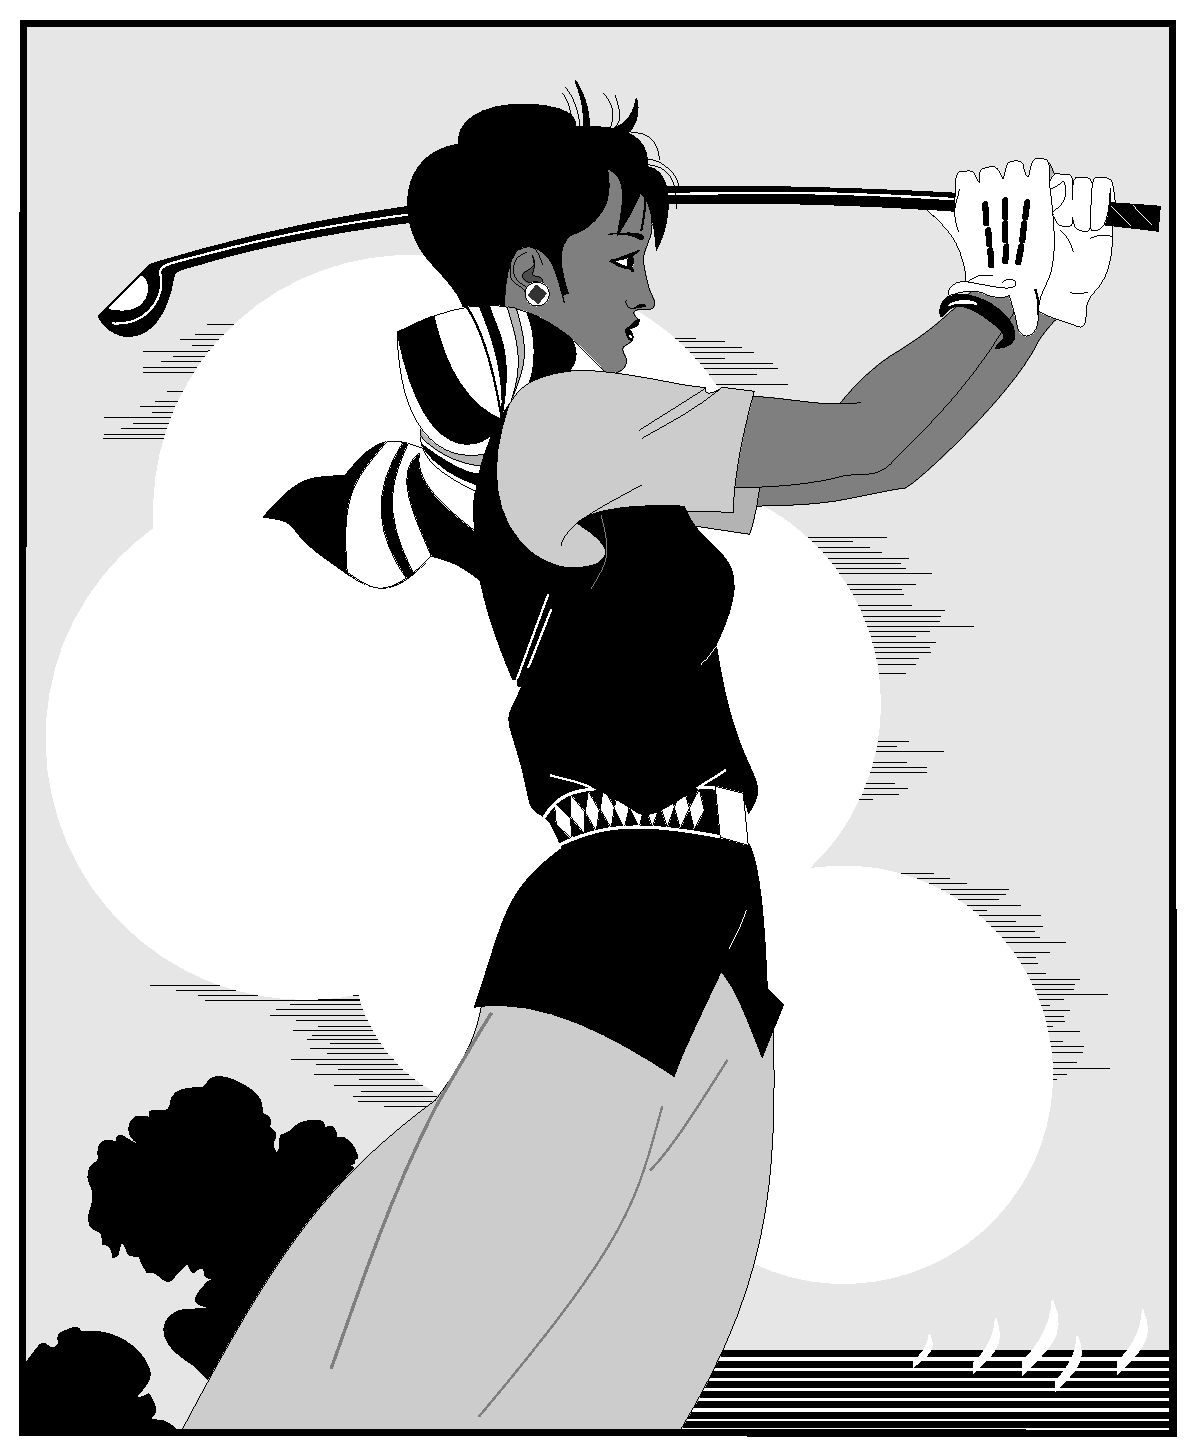
\includegraphics[width = 0.4\textwidth]{golfer}
\bicaption[golfer1]{}{打高尔夫球球的人(博士论文双语题注)}{Fig.$\!$}{The person playing golf (Doctoral thesis)}
\end{figure}

每个图均应有图题(由图序和图名组成),图题不宜有标点符号,图名在图序之后空1个半
角字符排写。图序按章编排,如第1章第一个插图的图号为“图1-1”。图题置于图下,硕士论
文只用中文,博士论文用中、英两种文字,居中书写,中文在上,要求中文用宋体5号字,
英文用Times New Roman 5号字。有图注或其它说明时应置于图题之上。引用图应注明出处
,在图题右上角加引用文献号。图中若有分图时,分图题置于分图之下或图题之下,可以只
用中文书写,分图号用a)、b)等表示。图中各部分说明应采用中文(引用的外文图除外)或
数字符号,各项文字说明置于图题之上(有分图时,置于分图题之上)。图中文字用宋体、
Times New Roman字体,字号尽量采用5号字(当字数较多时可用小5号字,以清晰表达为原
则,但在一个插图内字号要统一)。同一图内使用文字应统一。图表中物理量、符号用斜体
。
\subsection{本硕论文题注}[Other picture example]
\begin{figure}[h]
\centering
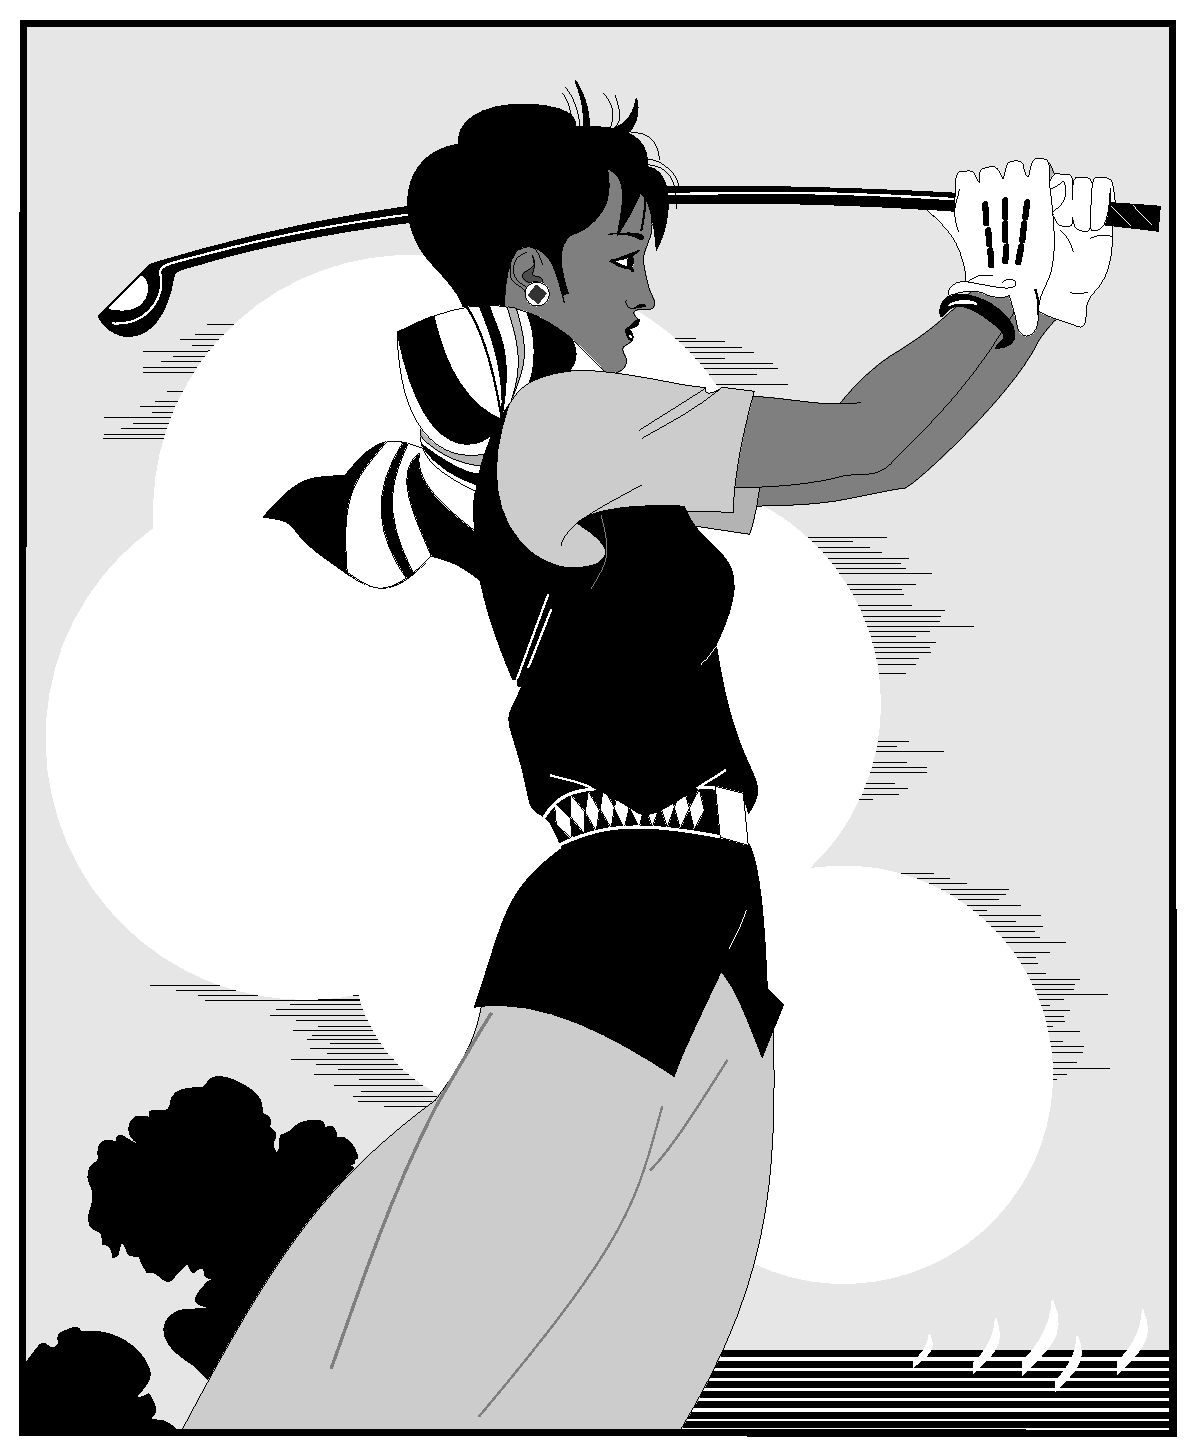
\includegraphics[width = 0.4\textwidth]{golfer}
\caption{打高尔夫球的人,硕士论文要求只用汉语}
\end{figure}

\subsection{并排图和子图}[Abreast-picture and Sub-picture example]
\subsubsection{并排图}[Abreast-picture example]

使用并排图时,需要注意对齐方式。默认情况是中部对齐。这里给出中部对齐、顶部对齐
、图片底部对齐三种常见方式。其中,底部对齐方式有一个很巧妙的方式,将长度比较小
的图放在左面即可。

\begin{figure}[htbp]
\centering
\begin{minipage}{0.4\textwidth}
\centering
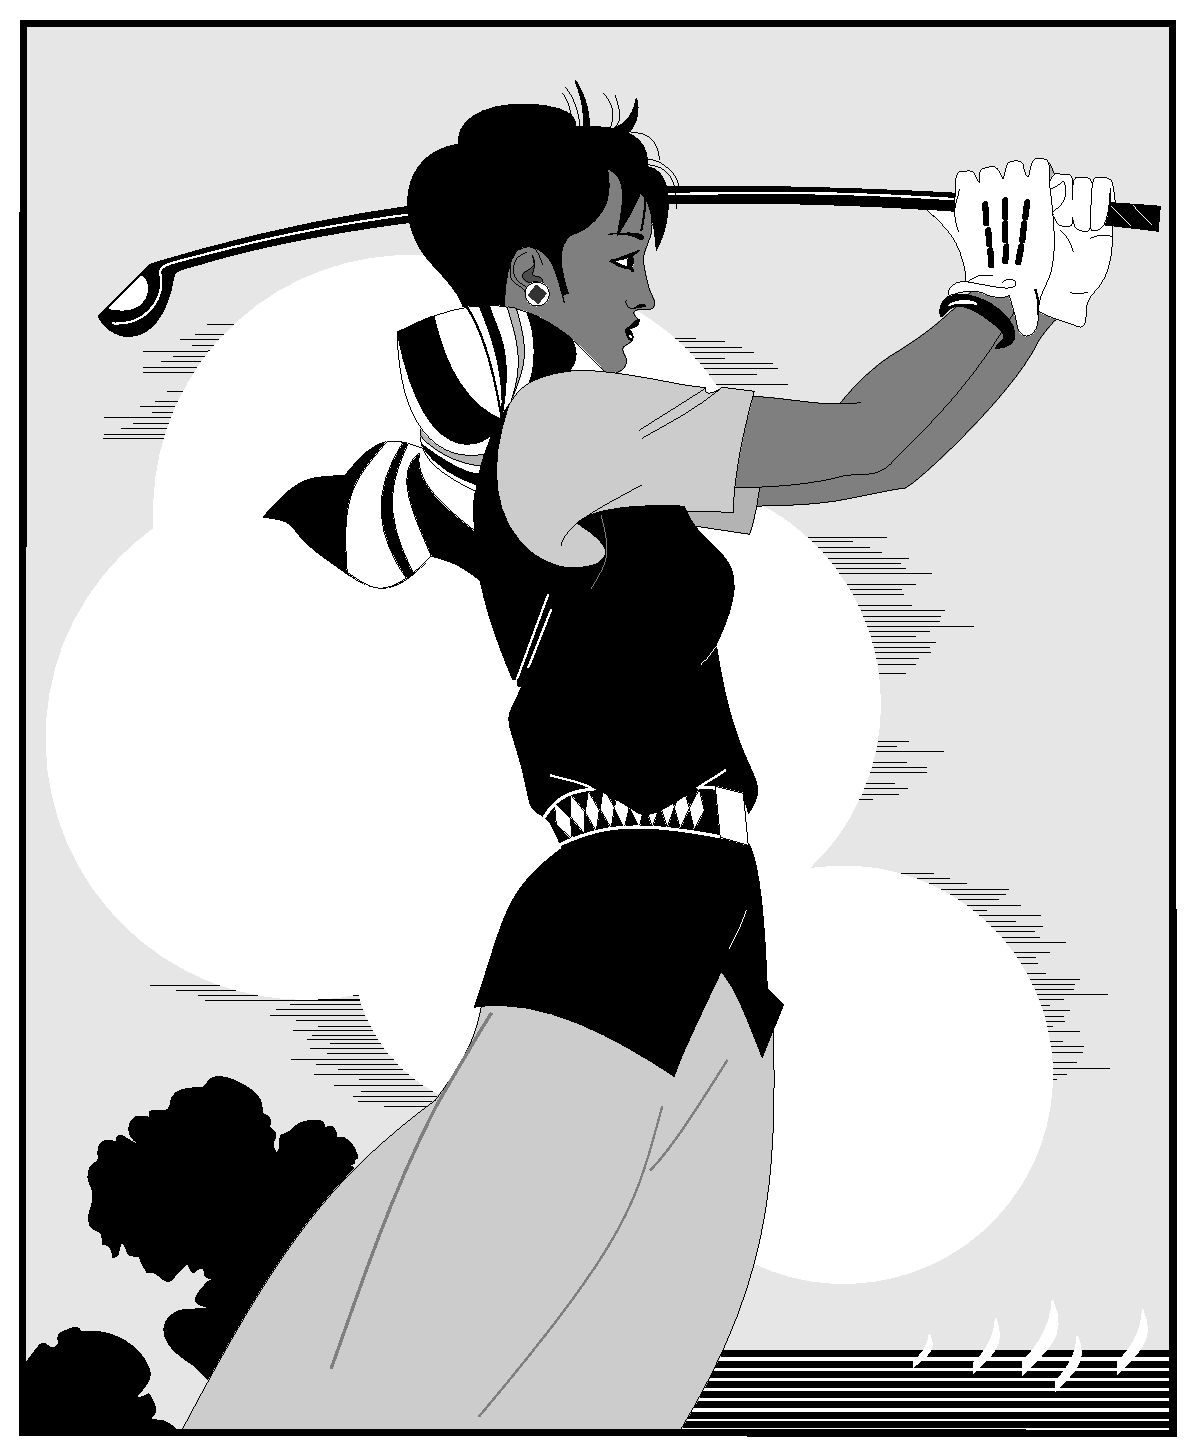
\includegraphics[width=\textwidth]{golfer}
\bicaption[golfer2]{}{打高尔夫球的人}{Fig.$\!$}{The person playing golf}
\end{minipage}
\centering
\begin{minipage}{0.4\textwidth}
\centering
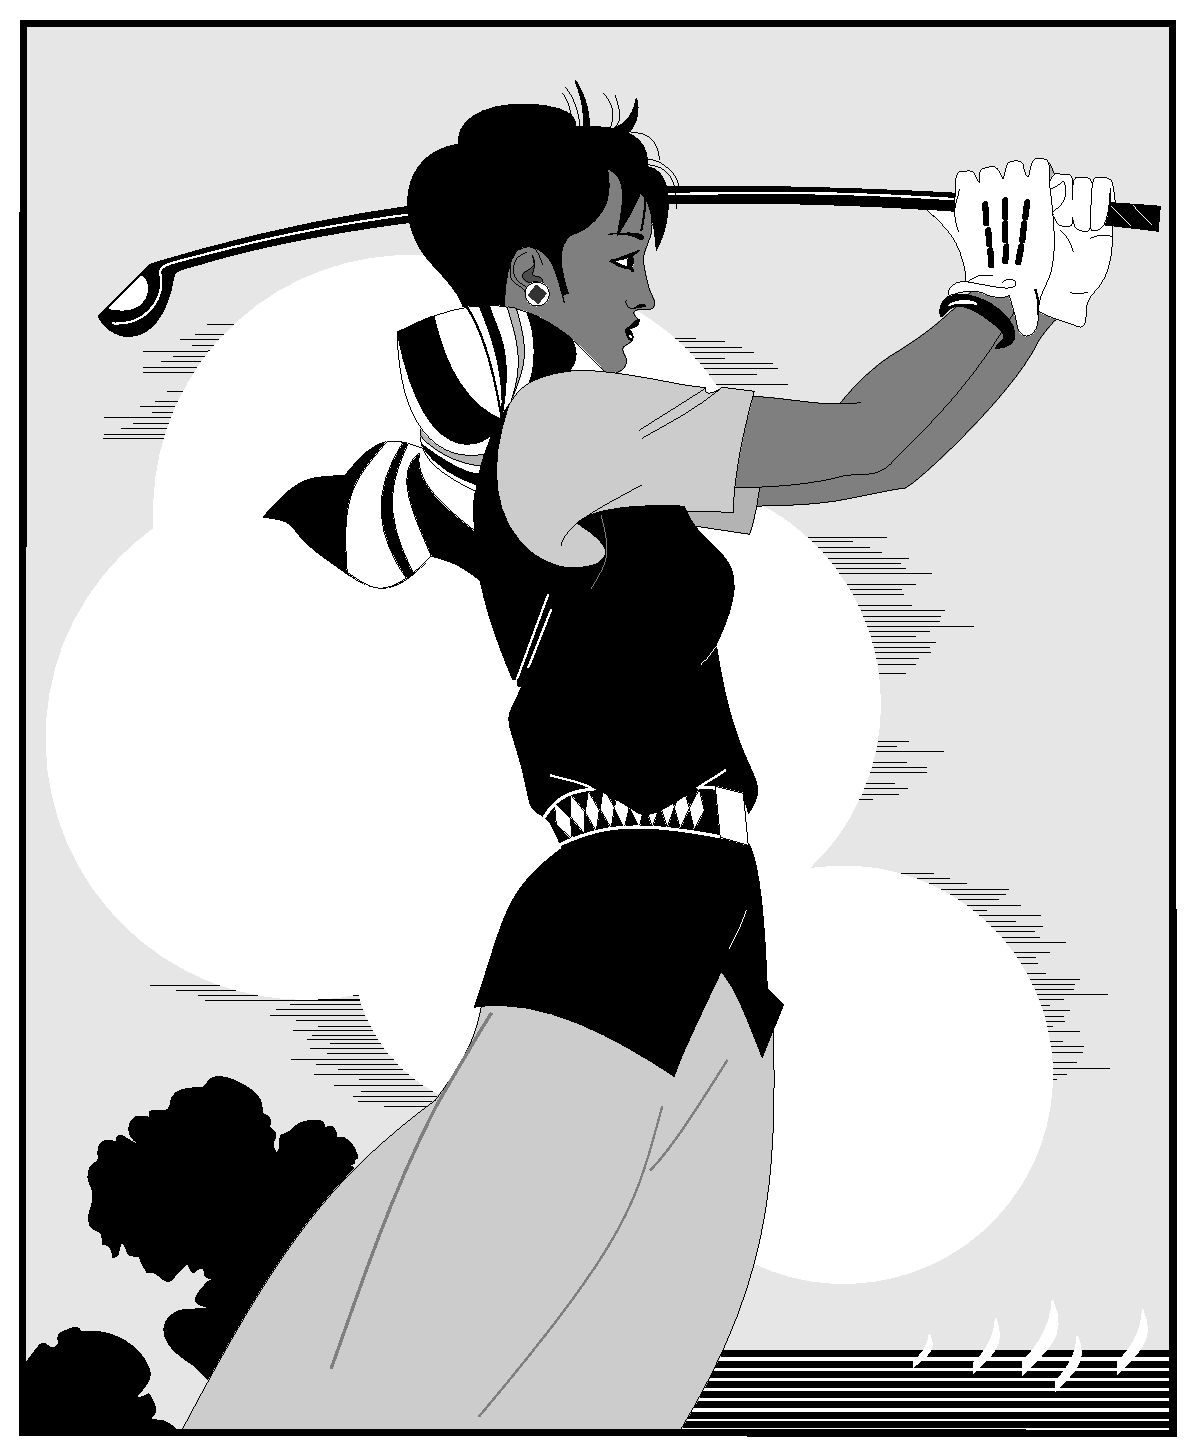
\includegraphics[width=\textwidth]{golfer}
\bicaption[golfer3]{}{打高尔夫球的人。注意,这里默认居中}{Fig.$\!$}{The person playing golf. Please note that, it is vertically center aligned by default.}
\end{minipage}
\end{figure}

\begin{figure}[htbp]
\centering
\begin{minipage}[t]{0.4\textwidth}
\centering
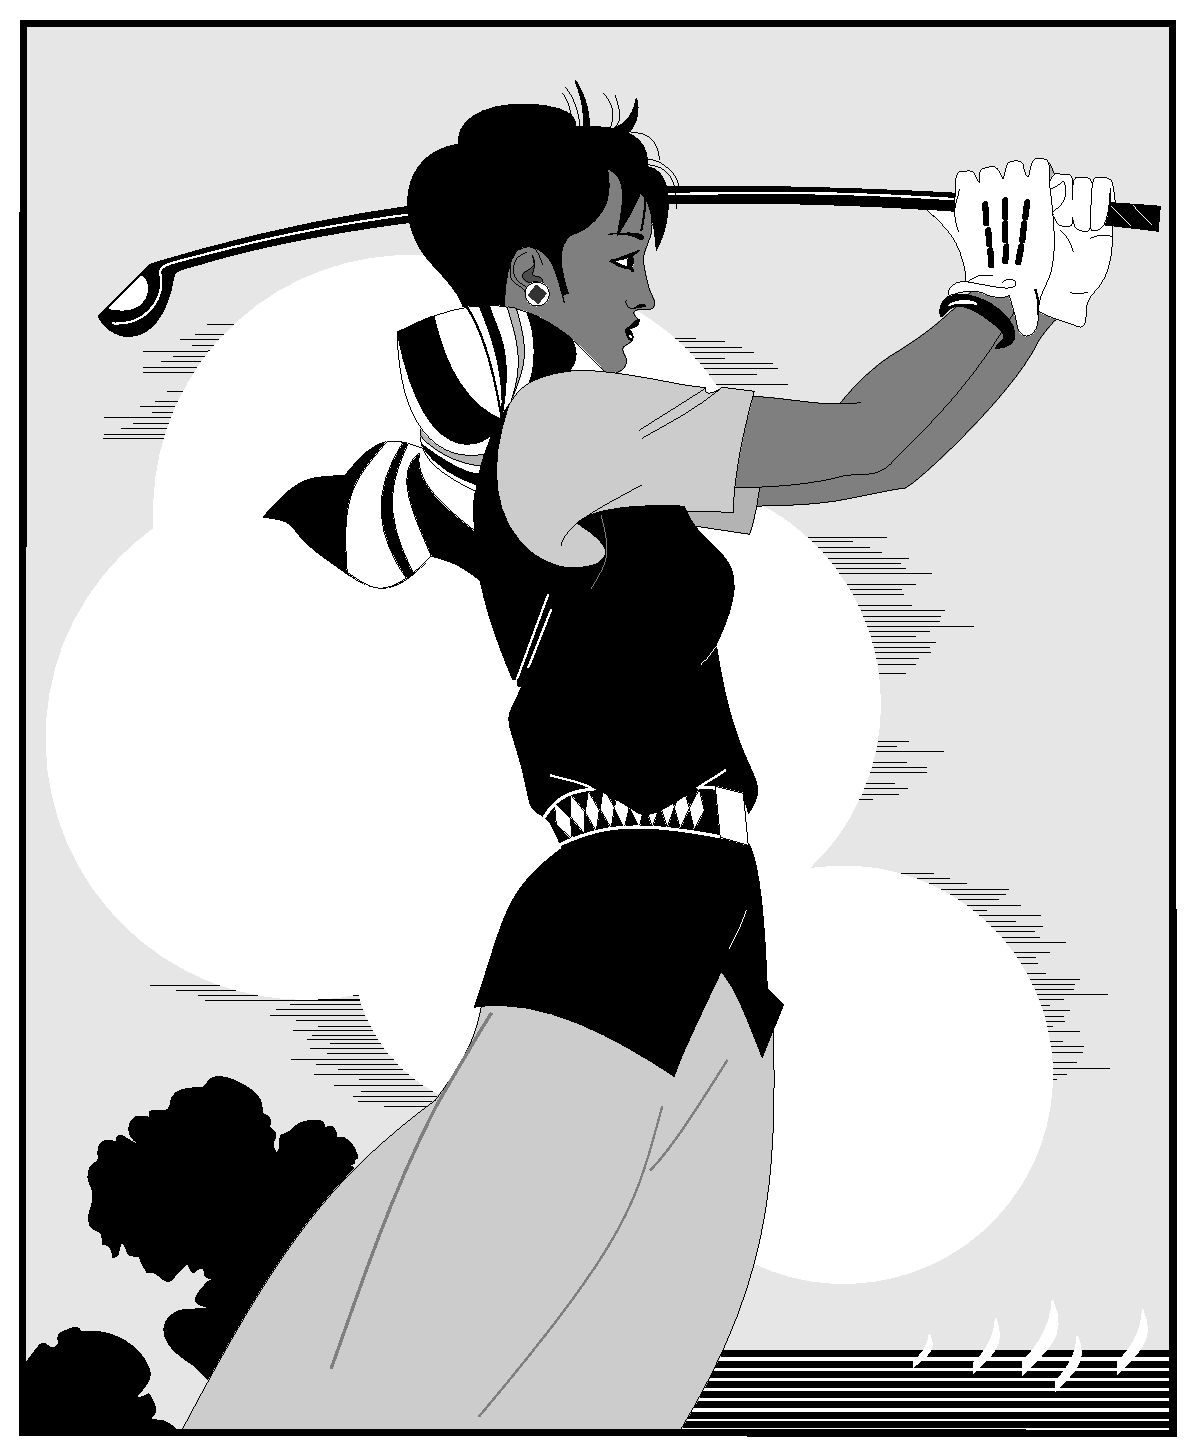
\includegraphics[width=\textwidth]{golfer}
\bicaption[golfer5]{}{打高尔夫球的人}{Fig.$\!$}{The person playing golf}
\end{minipage}
\centering
\begin{minipage}[t]{0.4\textwidth}
\centering
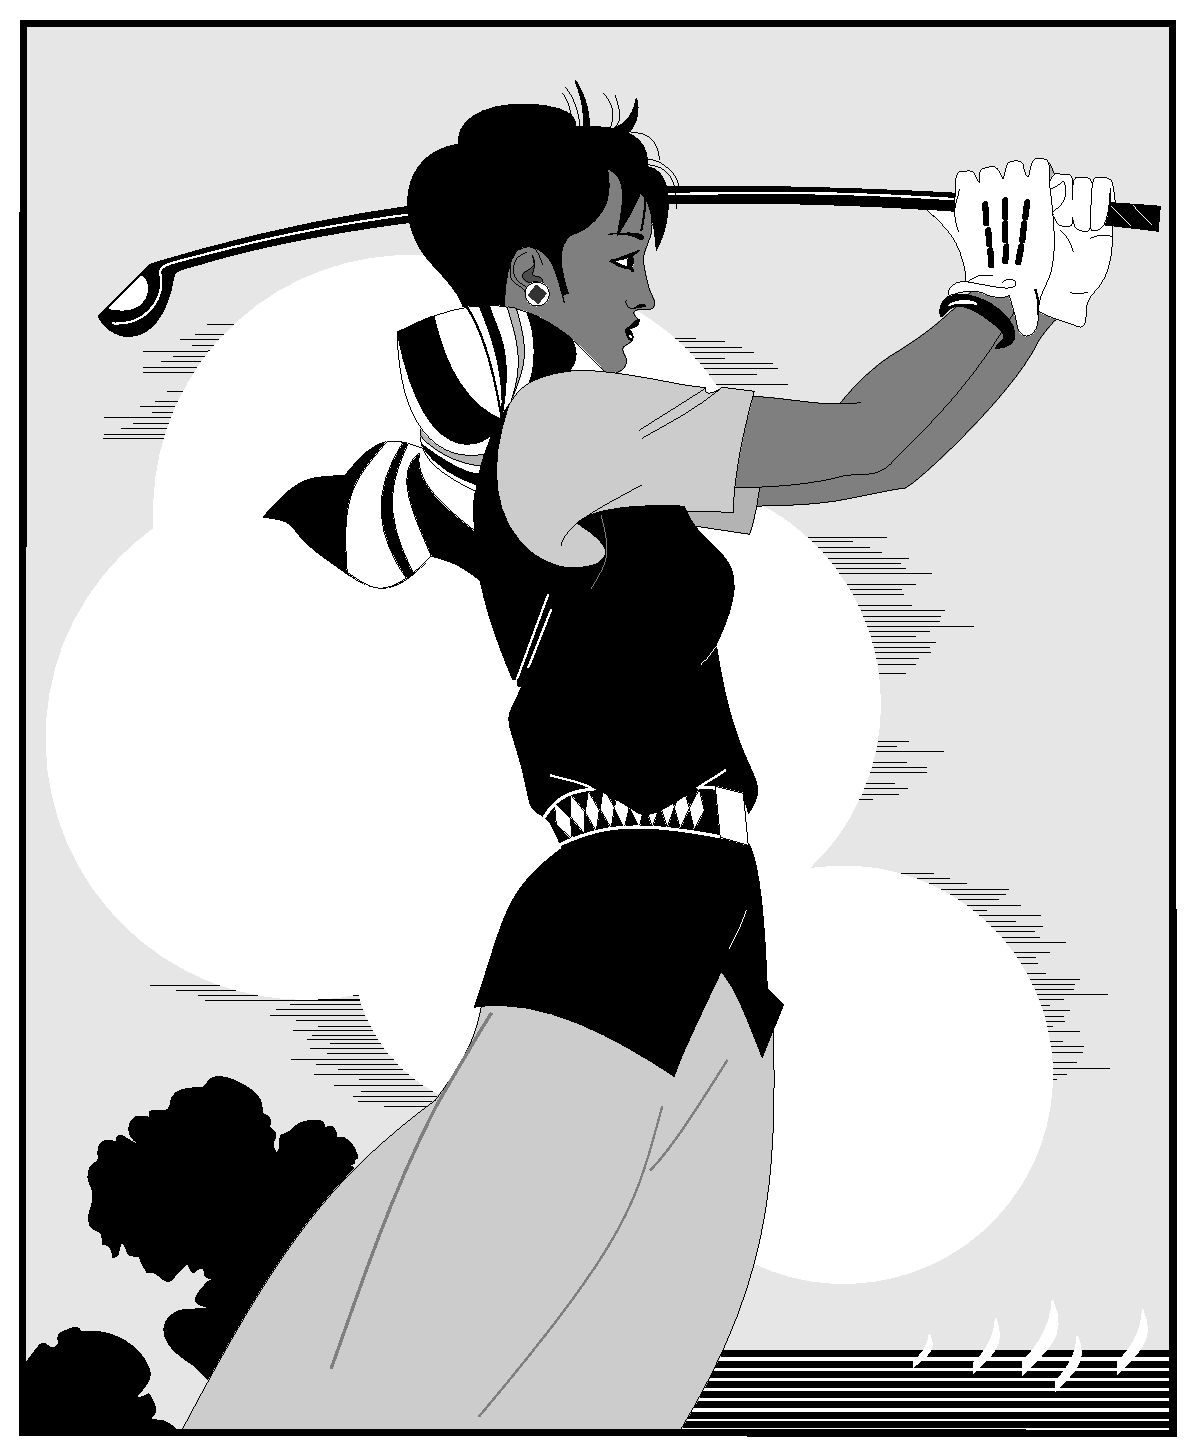
\includegraphics[width=\textwidth]{golfer}
\bicaption[golfer8]{}{打高尔夫球的人。注意,此图是顶部对齐}{Fig.$\!$}{The person playing golf. Please note that, it is vertically top aligned.}
\end{minipage}
\end{figure}

\begin{figure}[htbp]
\centering
\begin{minipage}[t]{0.4\textwidth}
\centering
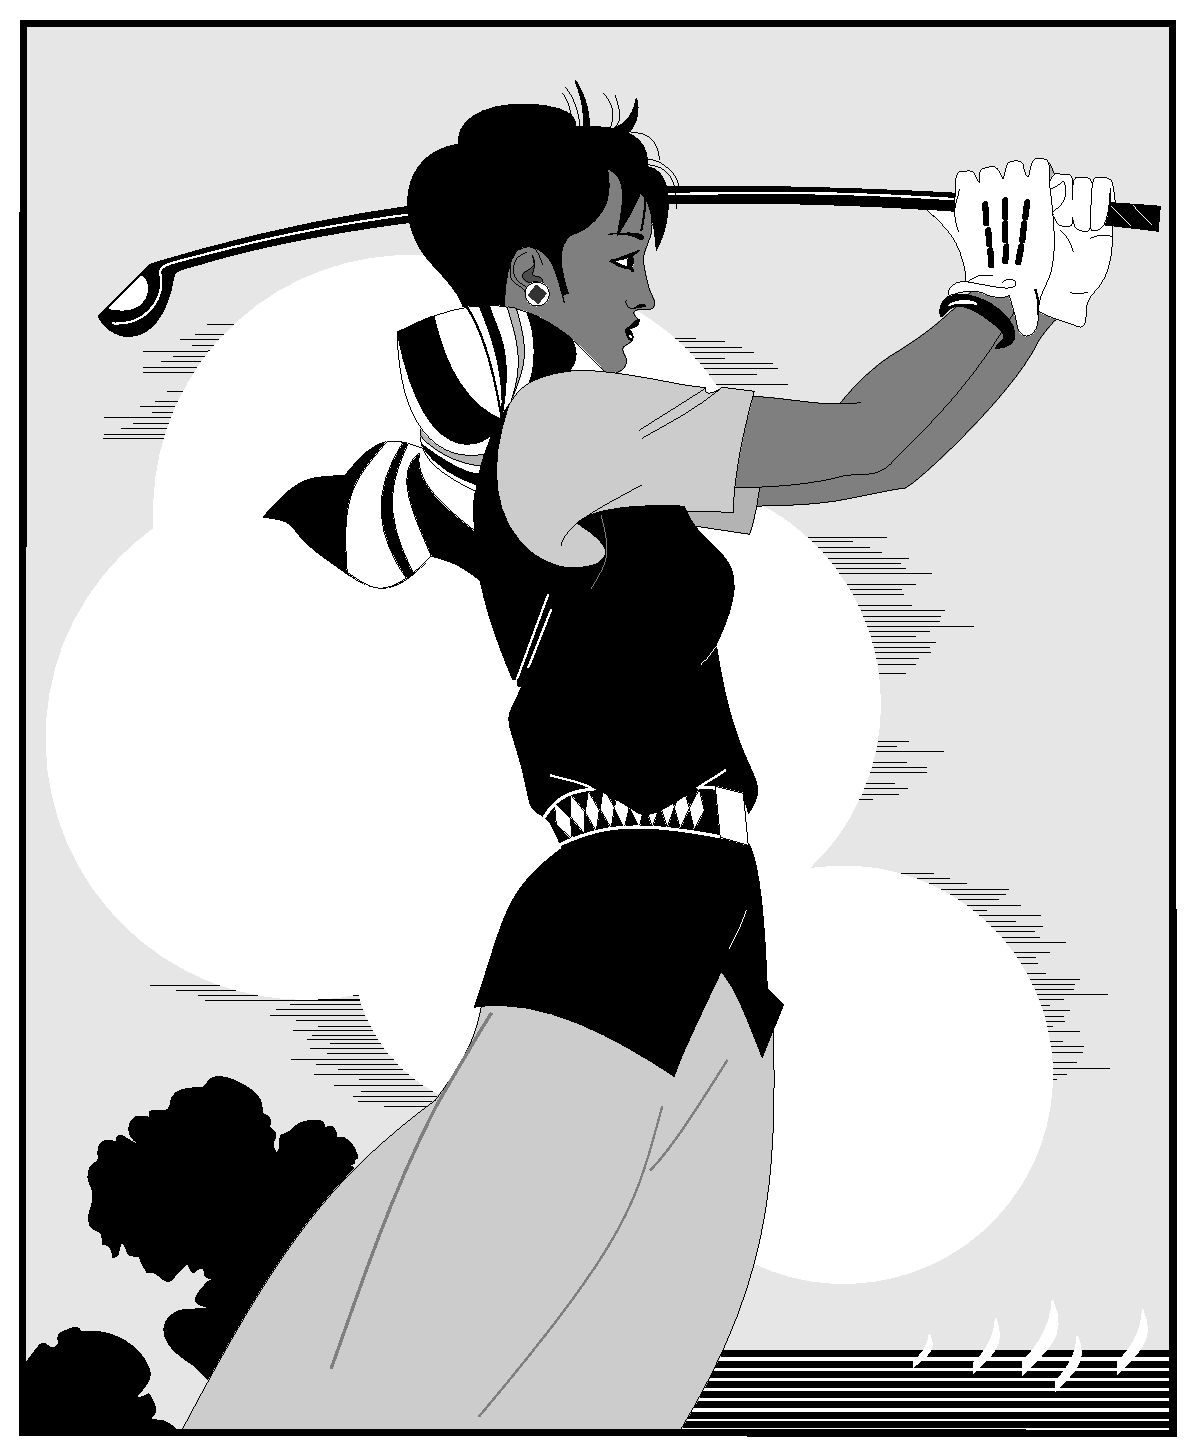
\includegraphics[width=\textwidth,height=\textwidth]{golfer}
\bicaption[golfer9]{}{打高尔夫球的人。注意,此图对齐方式是图片底部对齐}{Fig.$\!$}{The person playing golf. Please note that, it is vertically bottom aligned for figure.}
\end{minipage}
\centering
\begin{minipage}[t]{0.4\textwidth}
\centering
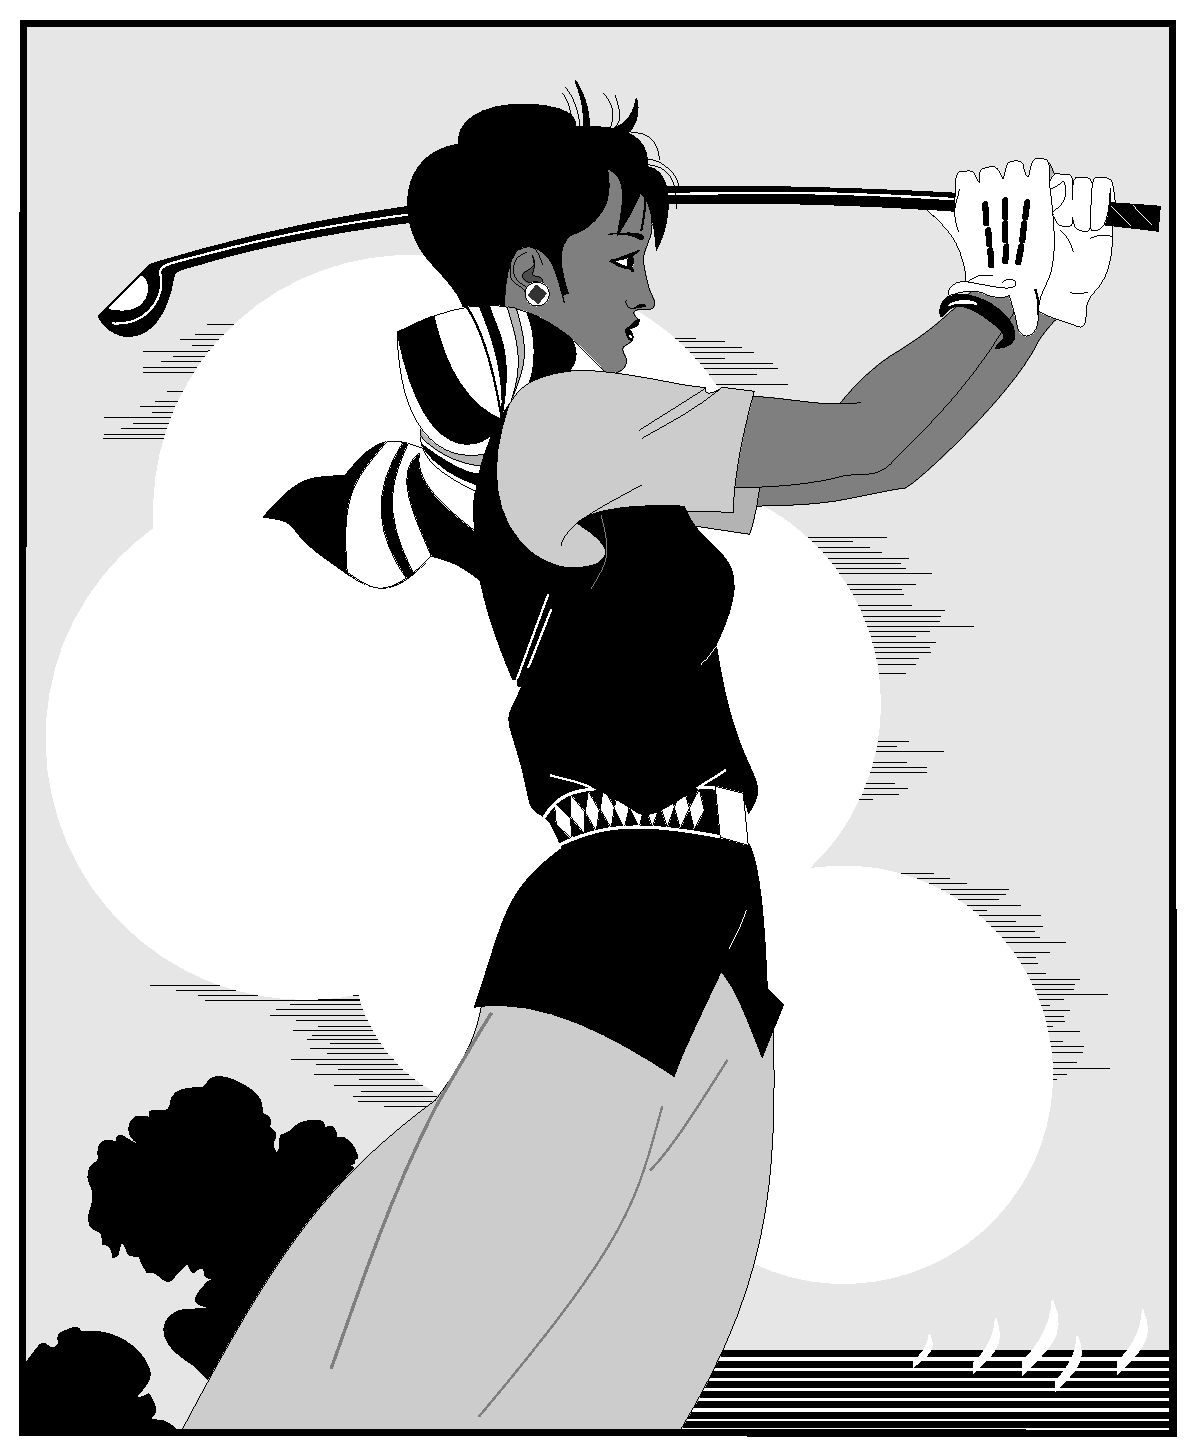
\includegraphics[width=\textwidth]{golfer}
\bicaption[golfer6]{}{打高尔夫球的人}{Fig.$\!$}{The person playing golf}
\end{minipage}
\end{figure}

\subsubsection{子图}[Sub-picture example]
注意:子图题注也可以只用中文。规范规定“分图题置于分图之下或图题之下”,但没有给出具体的格式要求。
没有要求的另外一个说法就是“无论什么格式都不对”。
所以只有在一个图中有标注“a),b)”,无法使用\cs{subfigure}的情况下,使用最后一个图例中的格式设置方法,否则不要使用。
为了应对“无论什么格式都不对”,这个子图图题使用“minipage”和“description”环境,宽度,对齐方式可以按照个人喜好自由设置,是否使用双语子图图题也可以自由设置。

\begin{figure}[!h]
\setlength{\subfigcapskip}{-1bp}
\centering
\begin{minipage}{\textwidth}
\centering
\subfigure{\label{golfer41}}\addtocounter{subfigure}{-2}
\subfigure[The person playing golf]{\subfigure[打高尔夫球的人~1]{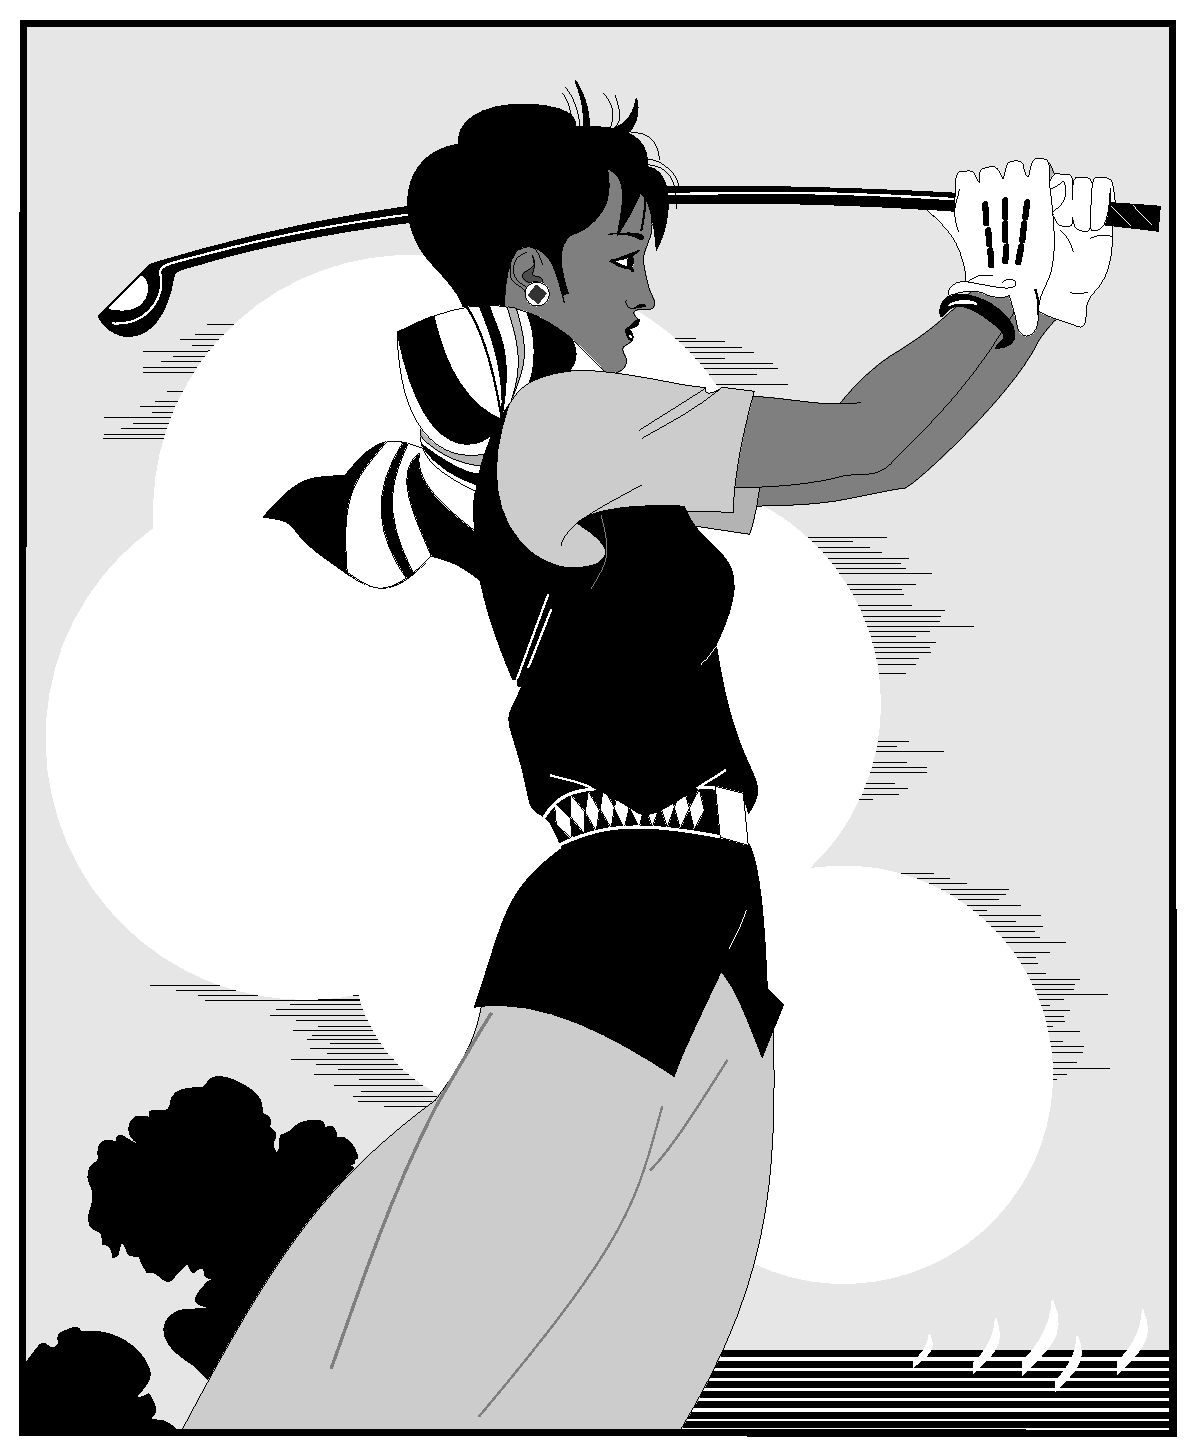
\includegraphics[width=0.4\textwidth]{golfer}}}
\hspace{2em}
\subfigure{\label{golfer42}}\addtocounter{subfigure}{-2}
\subfigure[The person playing golf]{\subfigure[打高尔夫球的人~2]{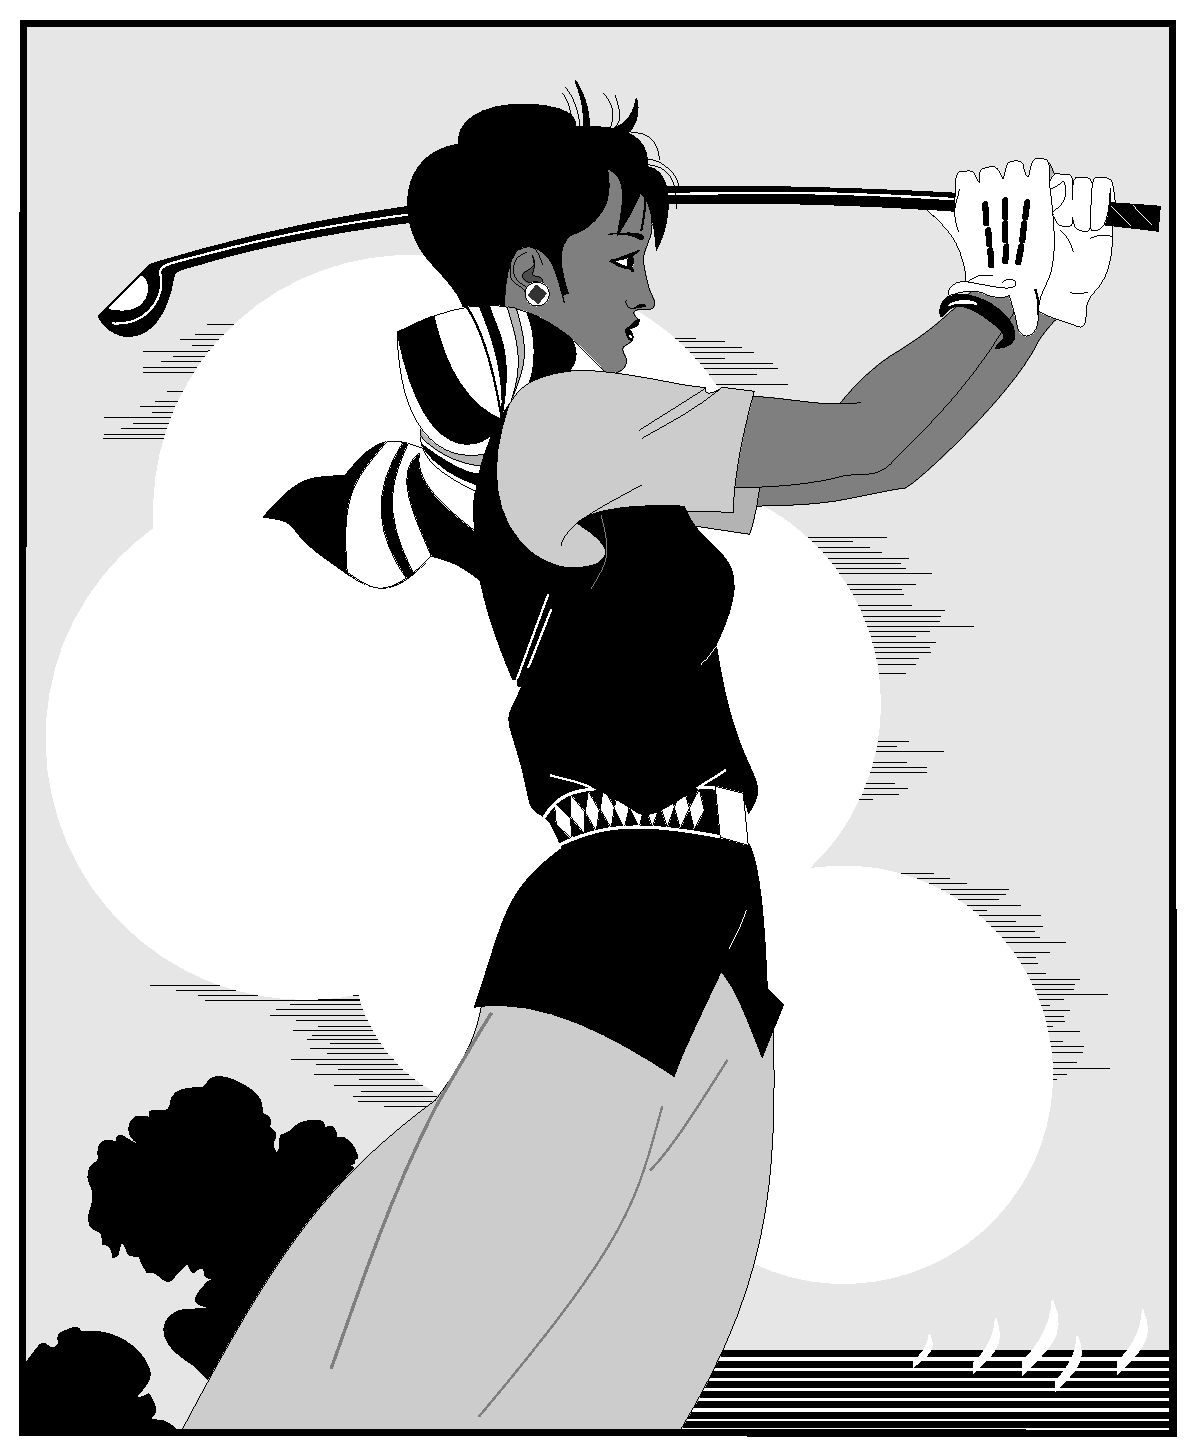
\includegraphics[width=0.4\textwidth]{golfer}}}
\end{minipage}
\centering
\begin{minipage}{\textwidth}
\centering
\subfigure{\label{golfer43}}\addtocounter{subfigure}{-2}
\subfigure[The person playing golf]{\subfigure[打高尔夫球的人~3]{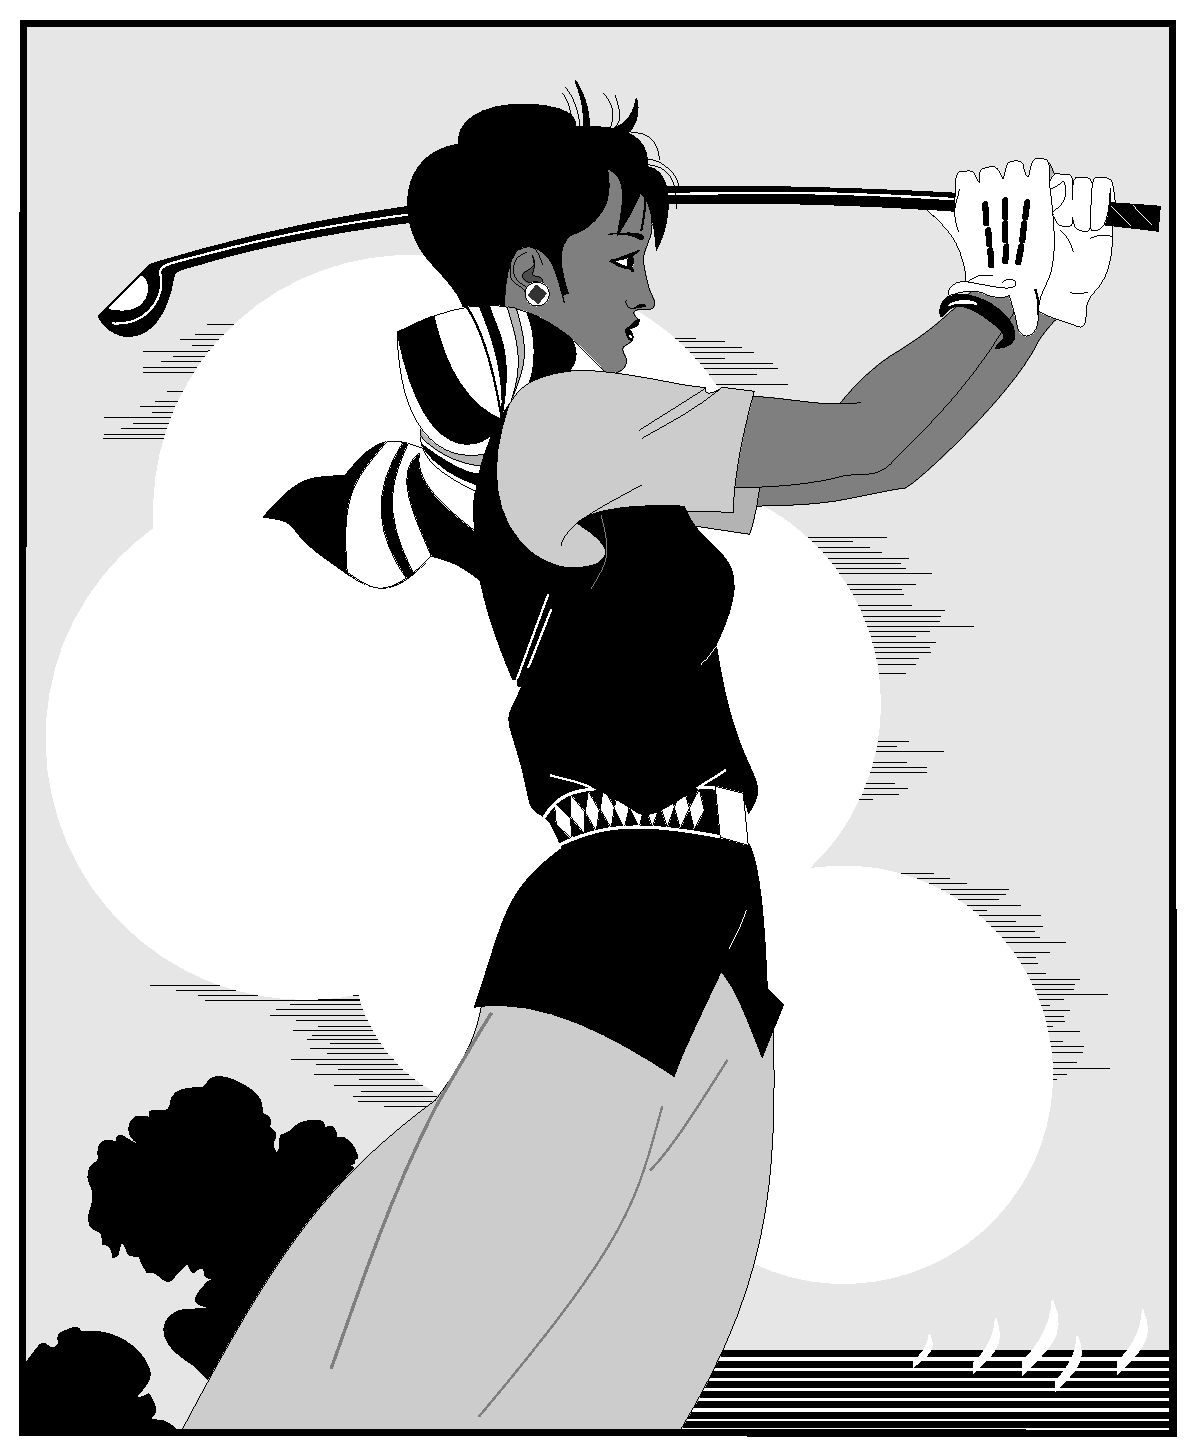
\includegraphics[width=0.4\textwidth]{golfer}}}
\hspace{2em}
\subfigure{\label{golfer44}}\addtocounter{subfigure}{-2}
\subfigure[The person playing golf. Here, 'hang indent' and 'center last line' are not stipulated in the regulation.]{\subfigure[打高尔夫球的人~4。注意,规范中没有明确规定要悬挂缩进、最后一行居中。]{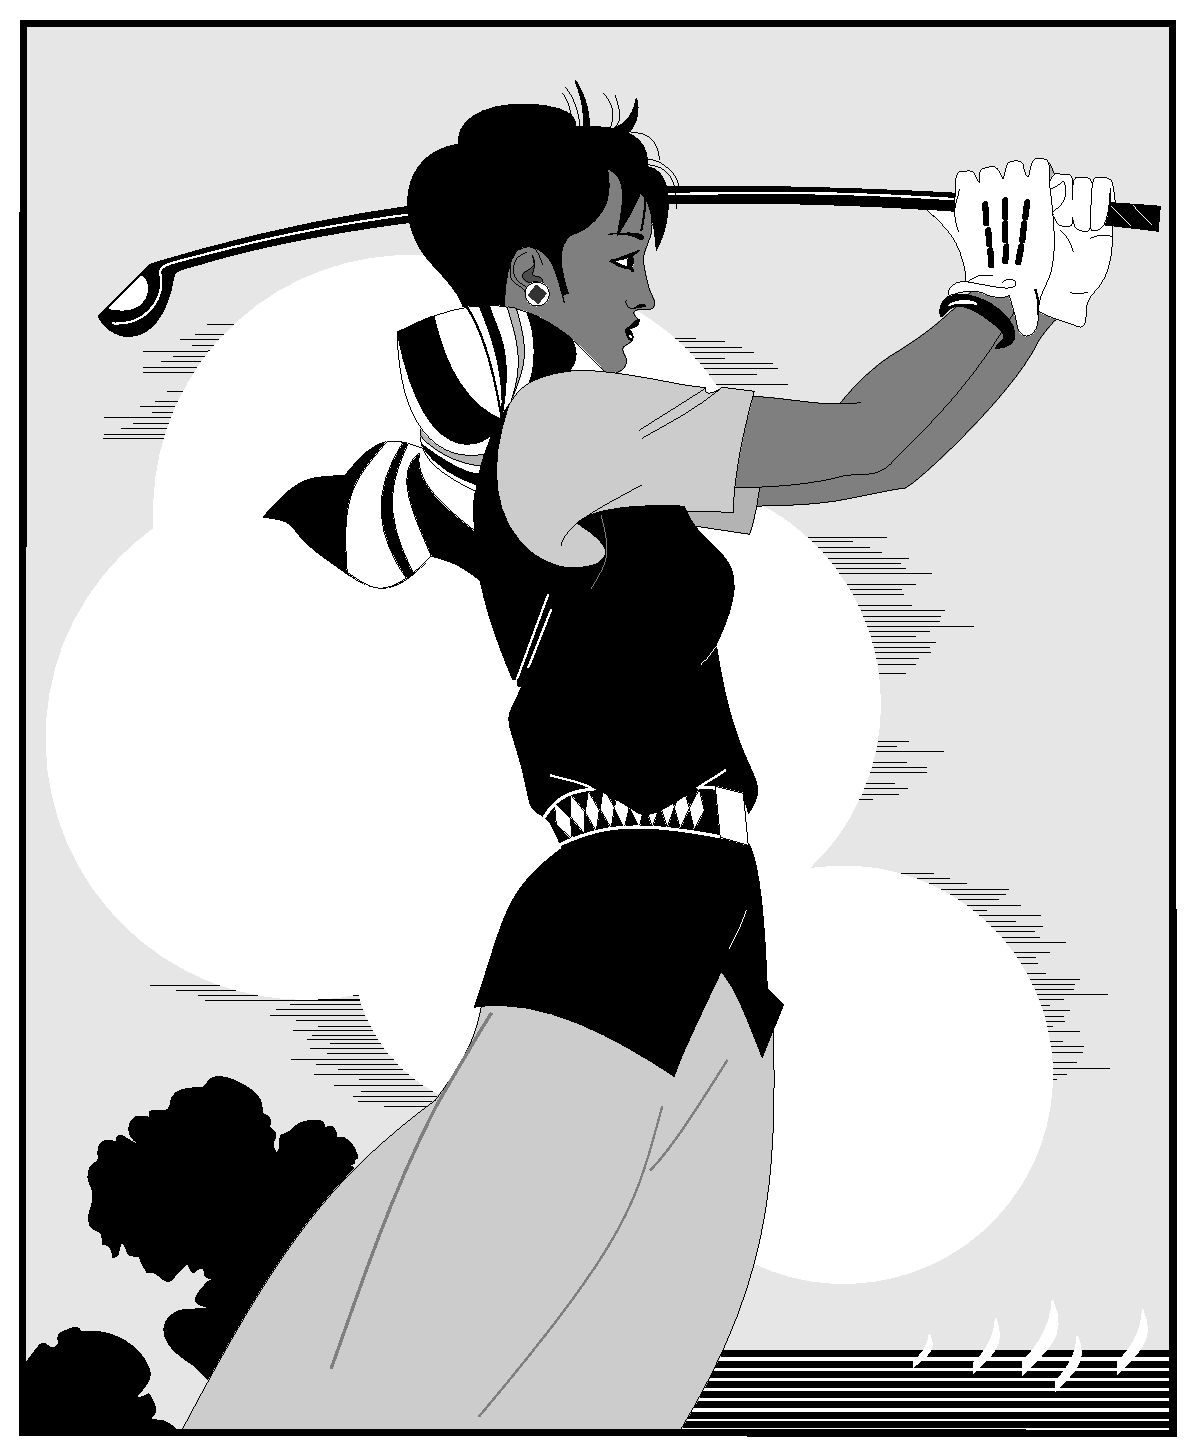
\includegraphics[width=0.4\textwidth]{golfer}}}
\end{minipage}
\vspace{0.2em}
\bicaption[golfer4]{}{打高尔夫球的人}{Fig.$\!$}{The person playing gol}
\end{figure}

\begin{figure}[t]
  \centering
  \begin{minipage}{.7\linewidth}
    \setlength{\subfigcapskip}{-1bp}
    \centering
    \begin{minipage}{\textwidth}
      \centering
      \subfigure{\label{golfer45}}\addtocounter{subfigure}{-2}
      \subfigure[The person playing golf]{\subfigure[打高尔夫球的人~1]{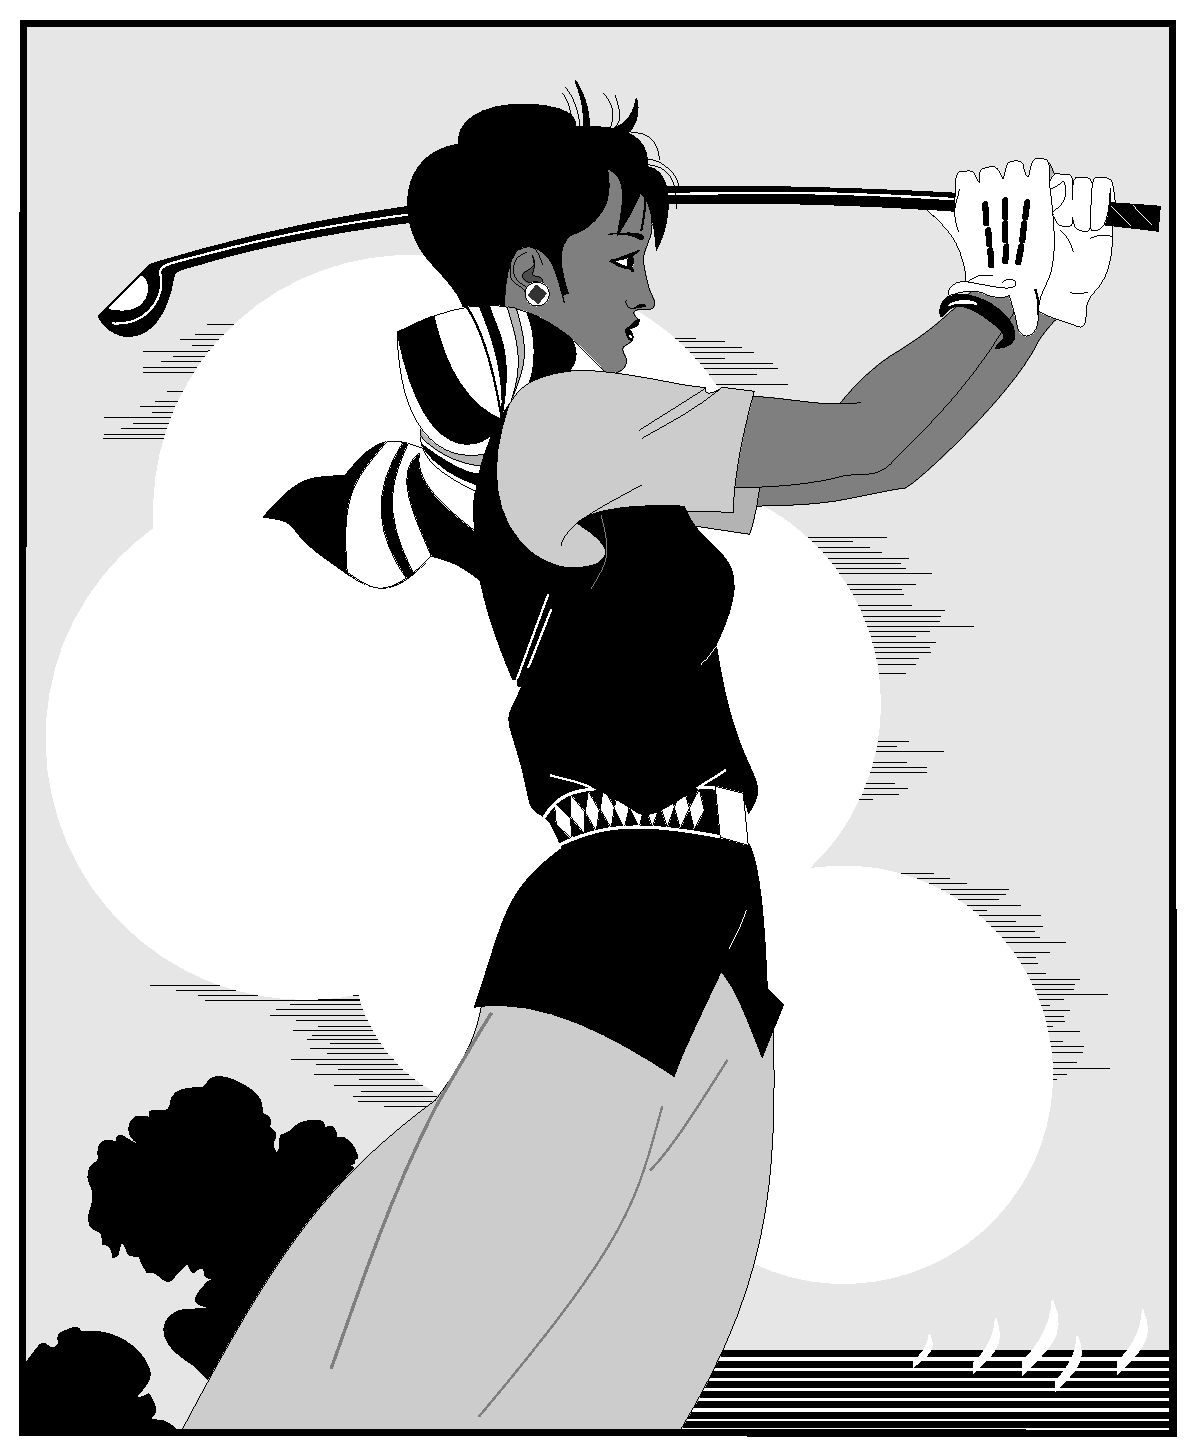
\includegraphics[width=0.4\textwidth]{golfer}}}
      \hspace{4em}
      \subfigure{\label{golfer46}}\addtocounter{subfigure}{-2}
      \subfigure[The person playing golf]{\subfigure[打高尔夫球的人~2]{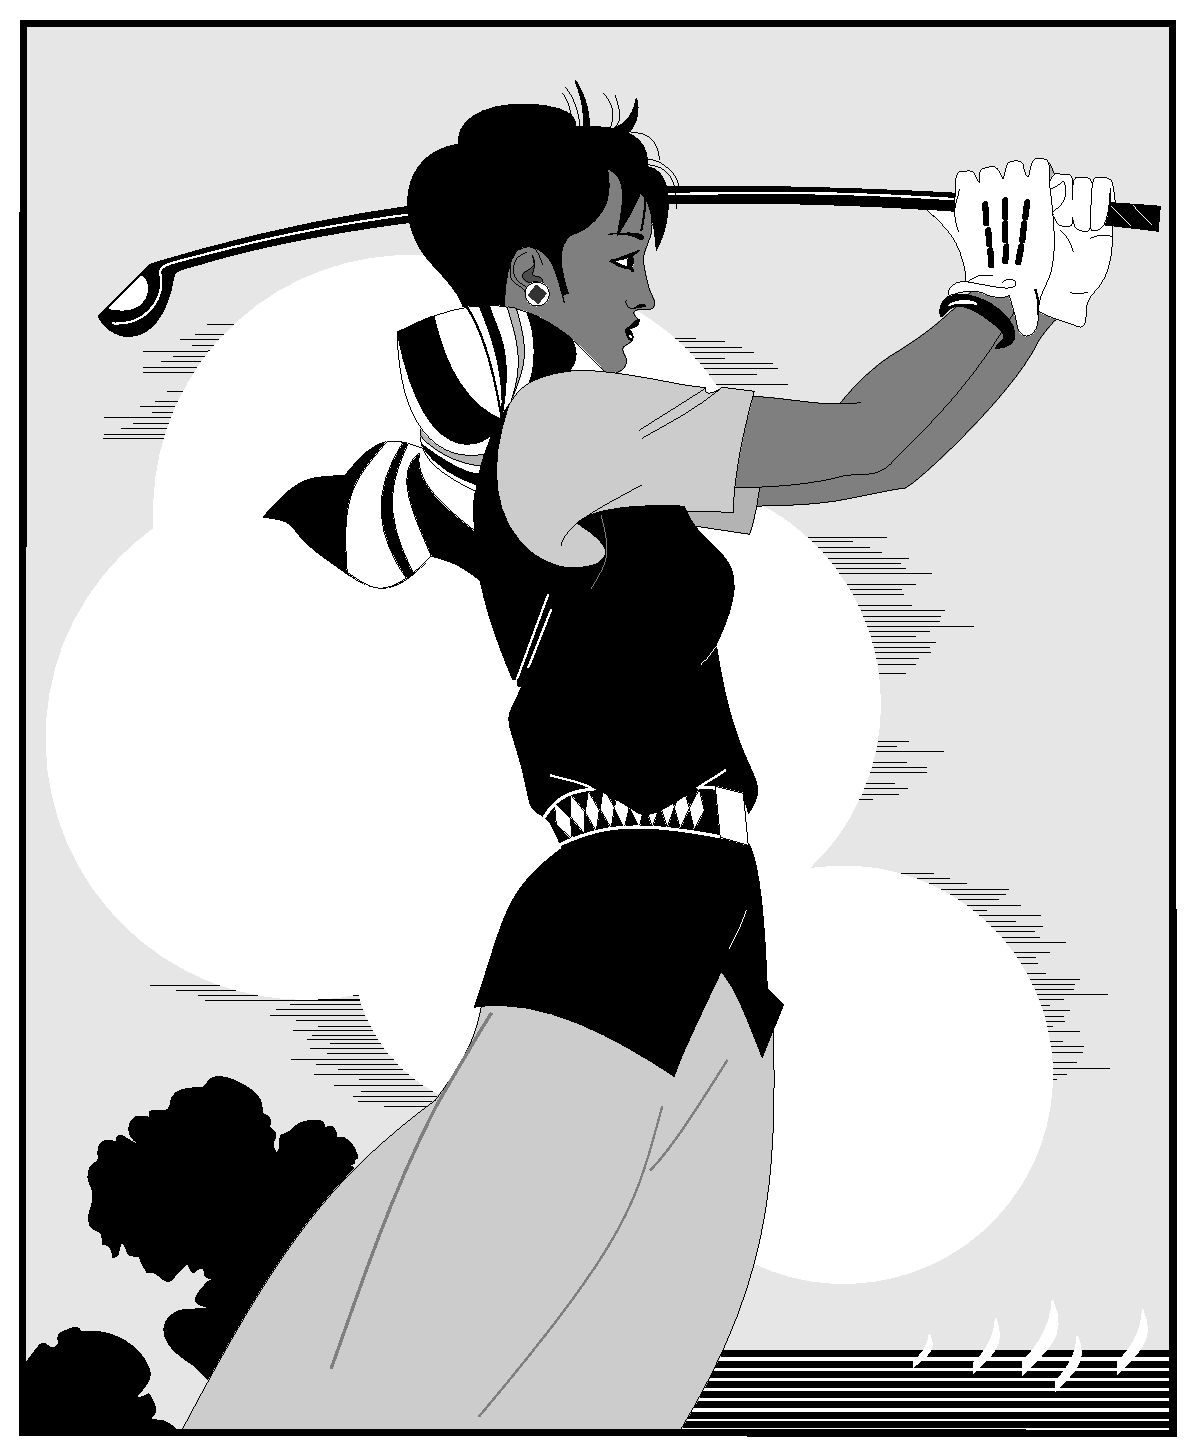
\includegraphics[width=0.4\textwidth]{golfer}}}
    \end{minipage}
    \vskip 0.2em
  \wuhao 注意:这里是中文图注添加位置(我工要求,图注在图题之上)。
    \vspace{0.2em}
\bicaption[golfer47]{}{打高尔夫球的人。注意,此处我工有另外一处要求,子图图题可以位于主图题之下。但由于没有明确说明位于下方具体是什么格式,所以这里不给出举例。}{Fig.$\!$}{The person playing golf. Please note that, although it is appropriate to put subfigures' captions under this caption as stipulated in regulation, but its format is not clearly stated.}
  \end{minipage}
\end{figure}

\begin{figure}[t]
\centering
\begin{tikzpicture}
	\node[anchor=south west,inner sep=0] (image) at (0,0) {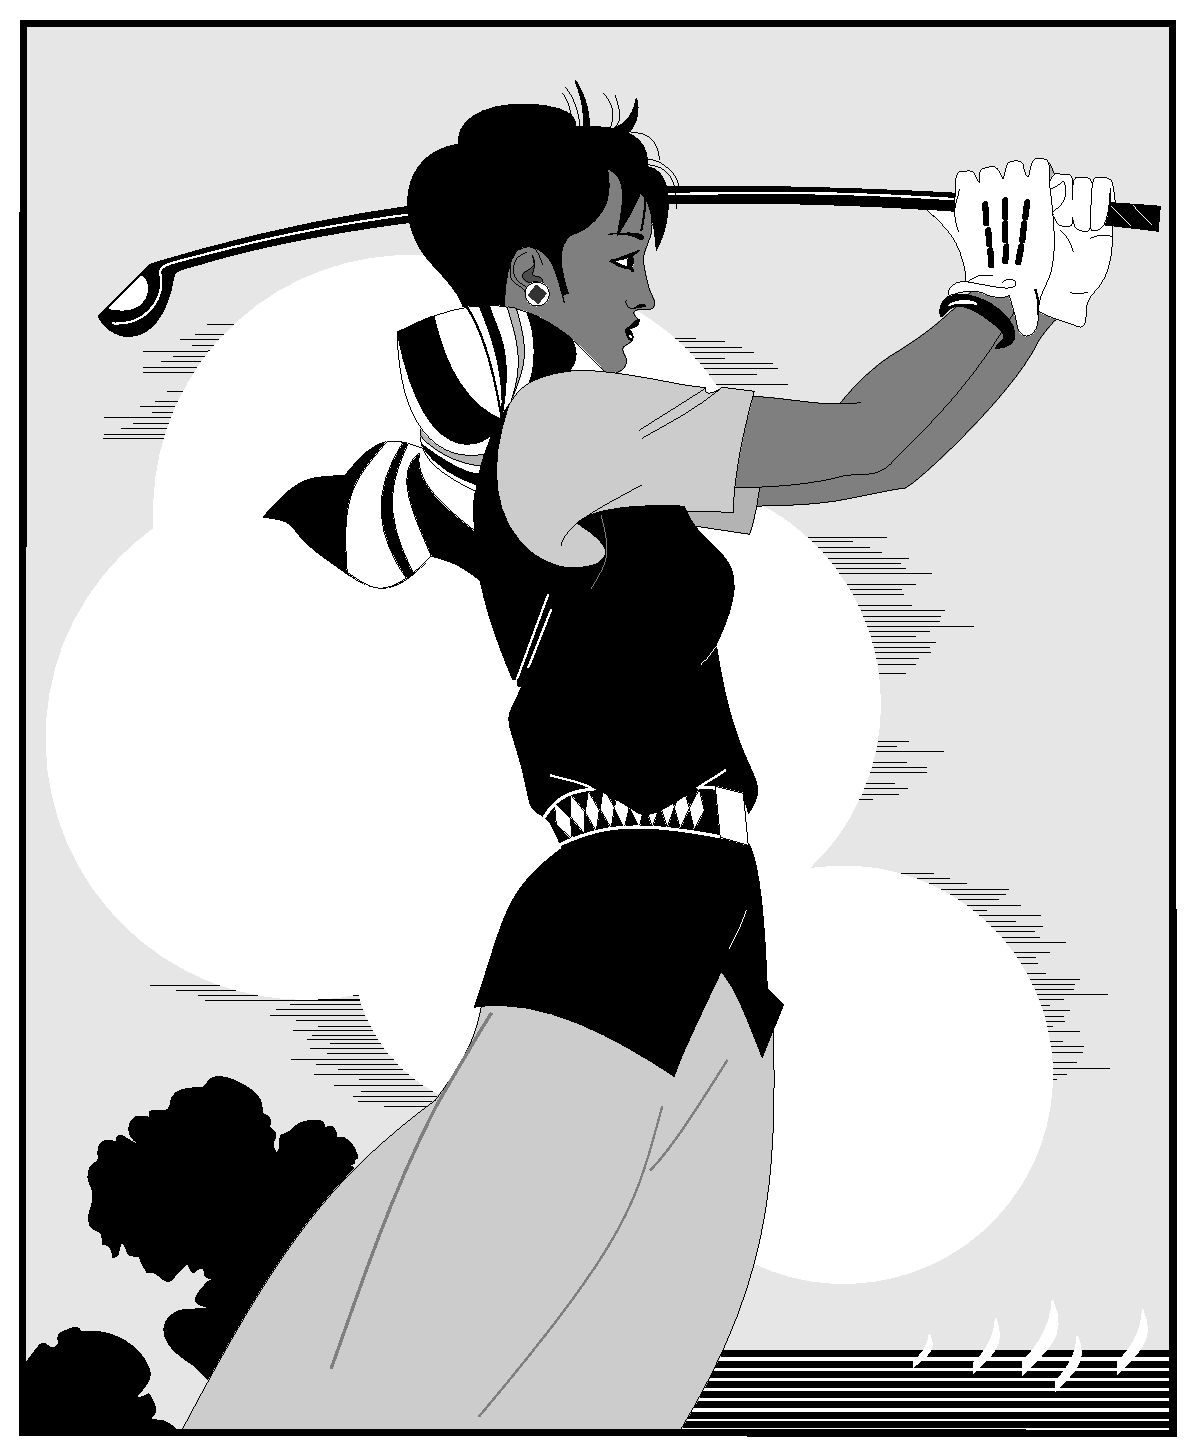
\includegraphics[width=0.3\textwidth]{golfer}};
	\begin{scope}[x={(image.south east)},y={(image.north west)}]
		\node at (0.3,0.5) {a)};
		\node at (0.8,0.2) {b)};
	\end{scope}
\end{tikzpicture}
\bicaption[golfer0]{}{打高尔夫球球的人(博士论文双语题注)}{Fig.$\!$}{The person playing golf (Doctoral thesis)}
\vskip -0.4em
 \hspace{2em}
\begin{minipage}[t]{0.3\textwidth}
\wuhao \setlist[description]{font=\normalfont}
	\begin{description}
		\item[a)]子图图题
	\end{description}
 \end{minipage}
 \hspace{2em}
 \begin{minipage}[t]{0.3\textwidth}
\wuhao \setlist[description]{font=\normalfont}
	\begin{description}
		\item[b)]子图图题
		\item[b)]Subfigure caption
	\end{description}
\end{minipage}
\end{figure}


\begin{figure}[!h]
	\centering
	\begin{sideways}
		\begin{minipage}{\textheight}
			\centering
			\fbox{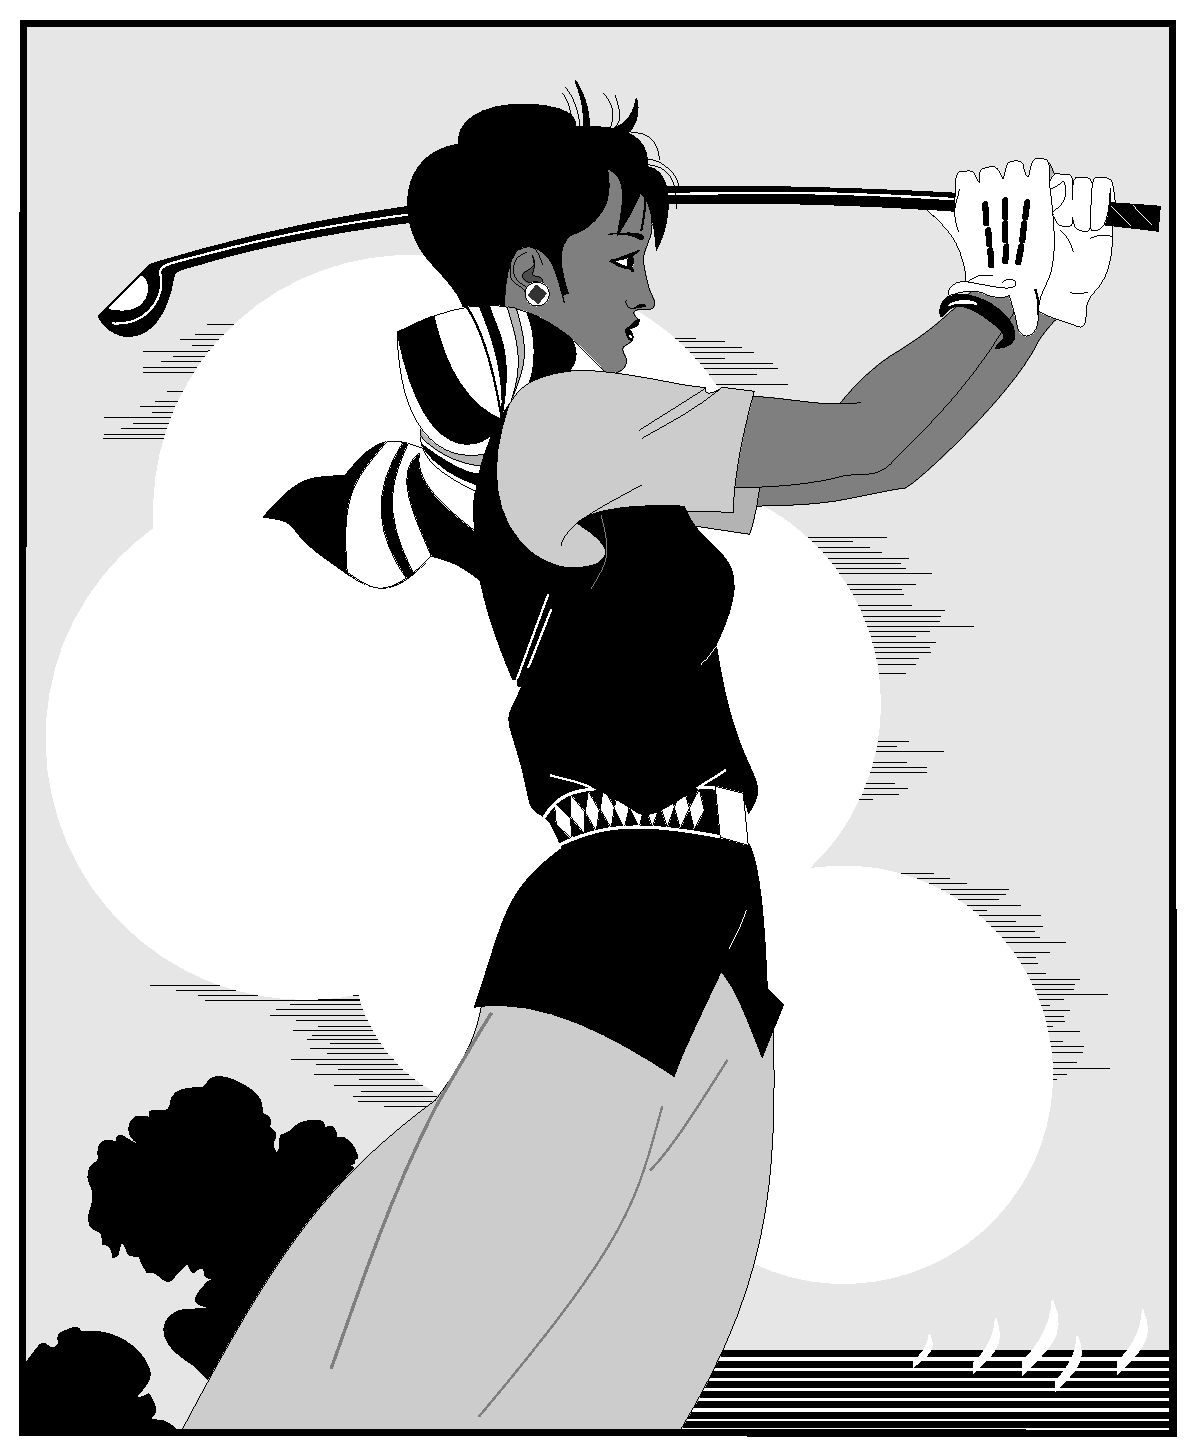
\includegraphics[width=0.2\textwidth]{golfer}}
			\fbox{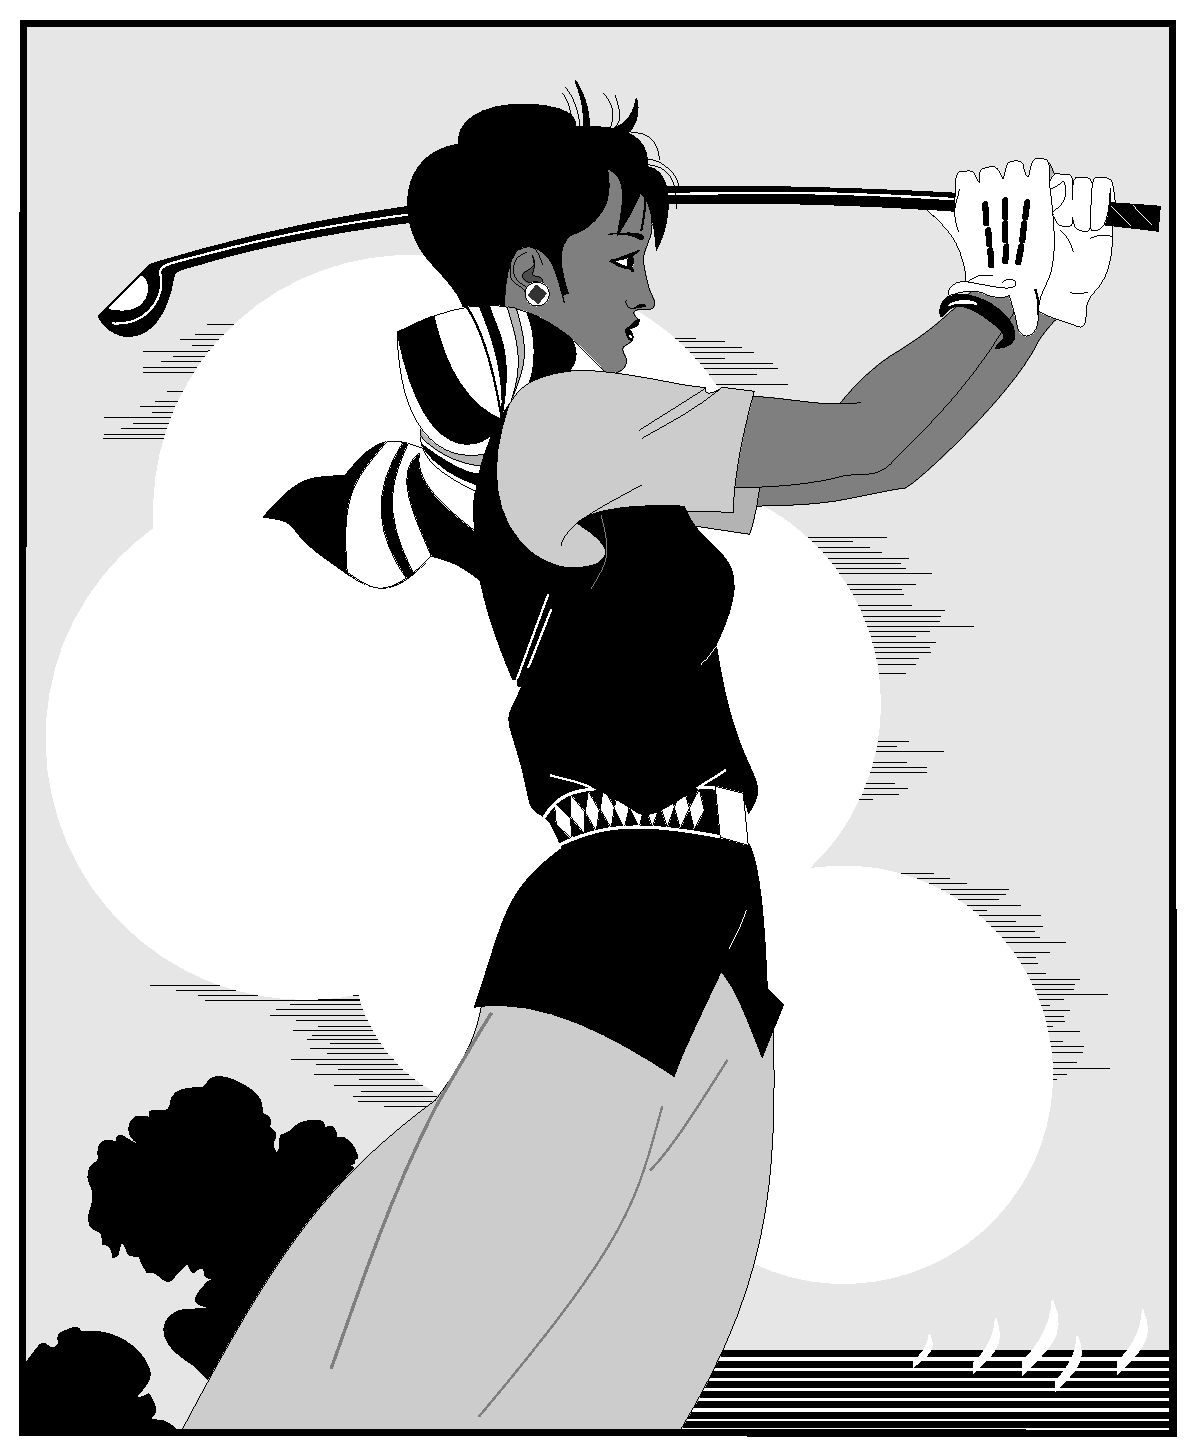
\includegraphics[width=0.2\textwidth]{golfer}}
			\fbox{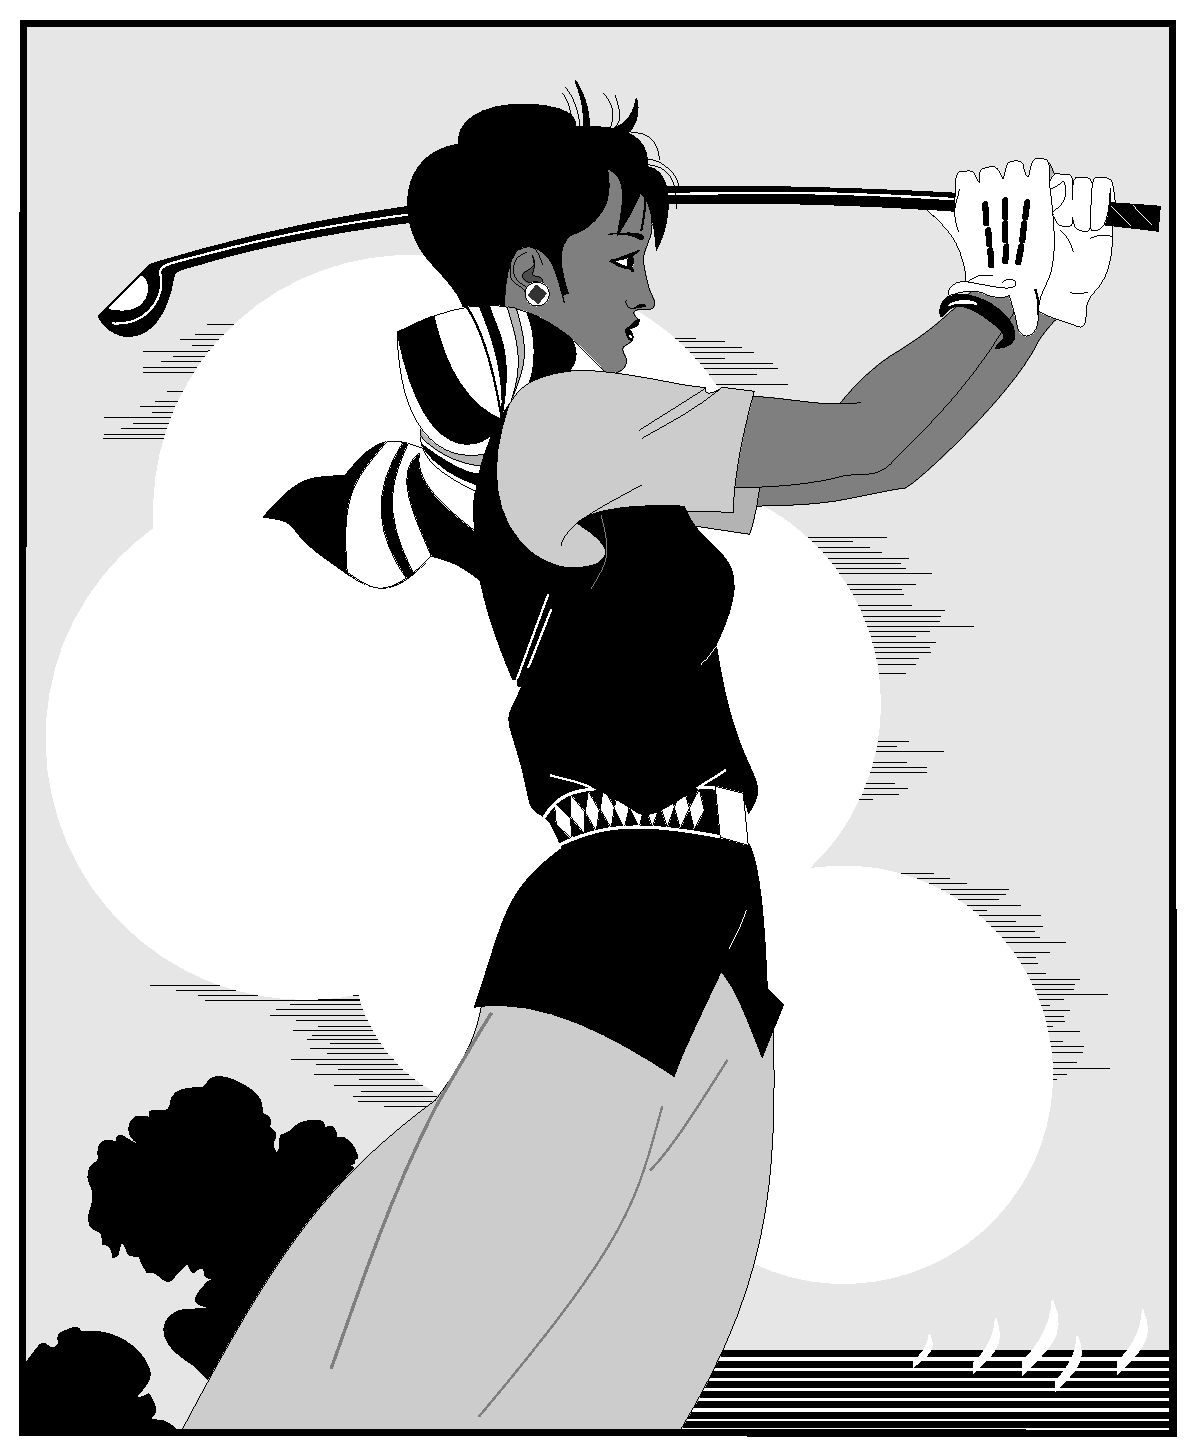
\includegraphics[width=0.2\textwidth]{golfer}}
			\fbox{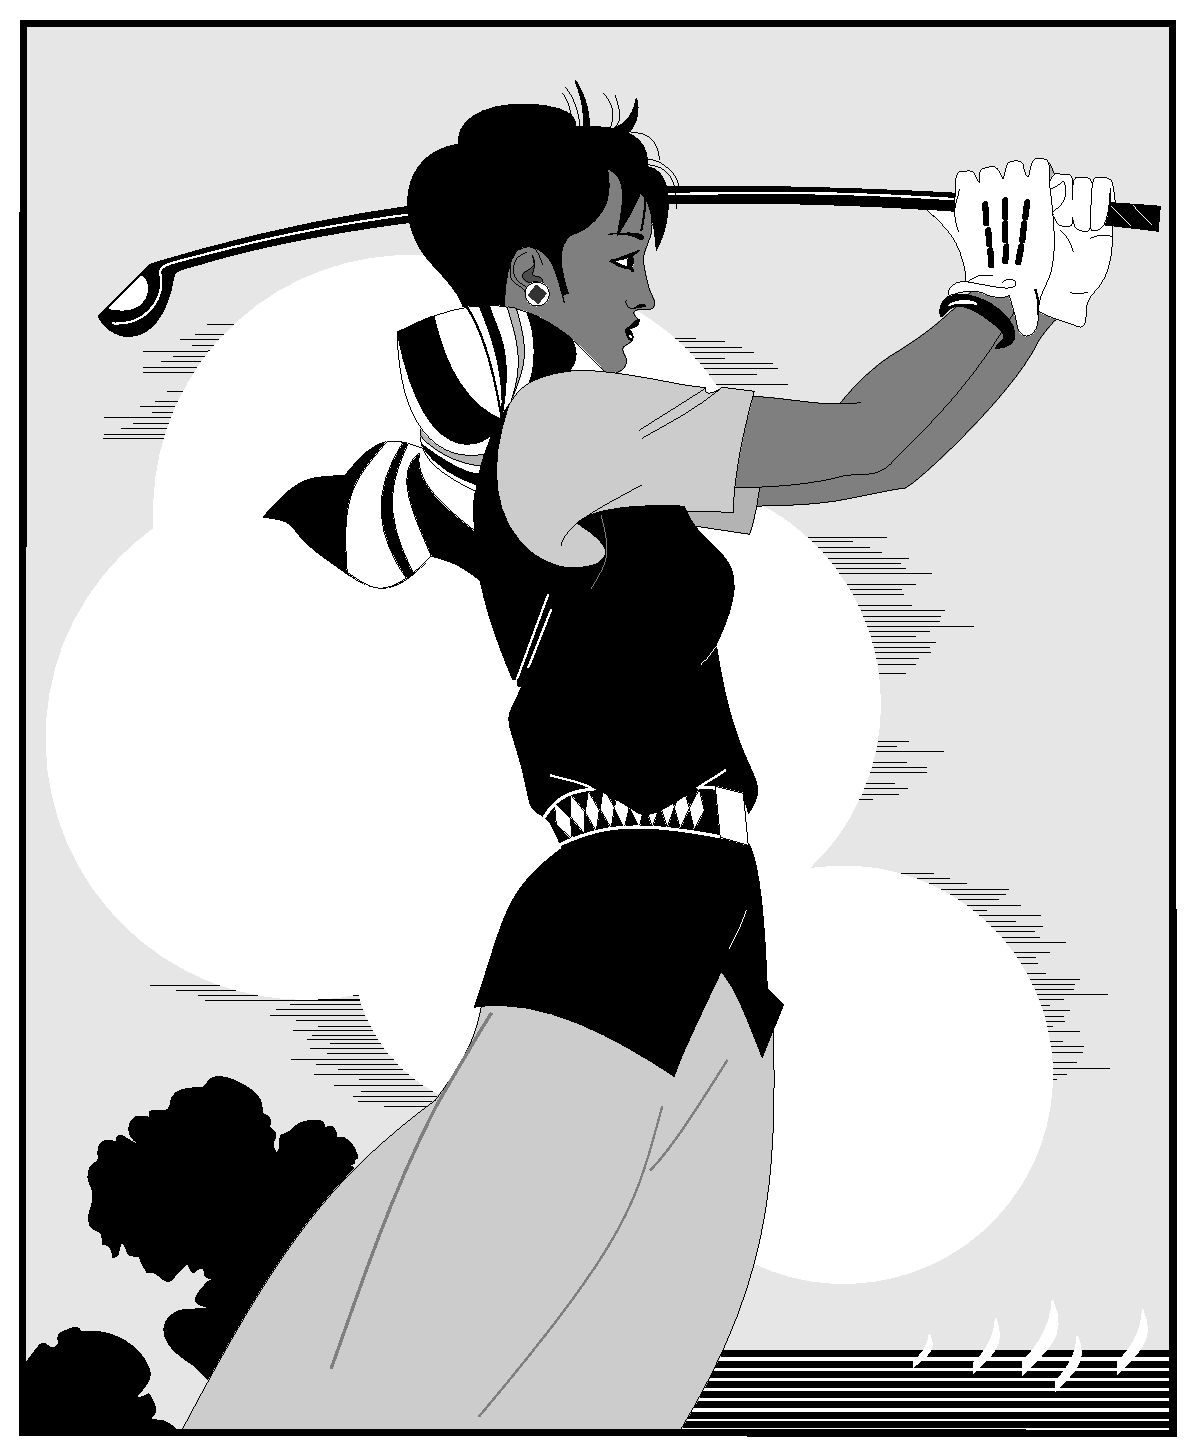
\includegraphics[width=0.2\textwidth]{golfer}}
			\fbox{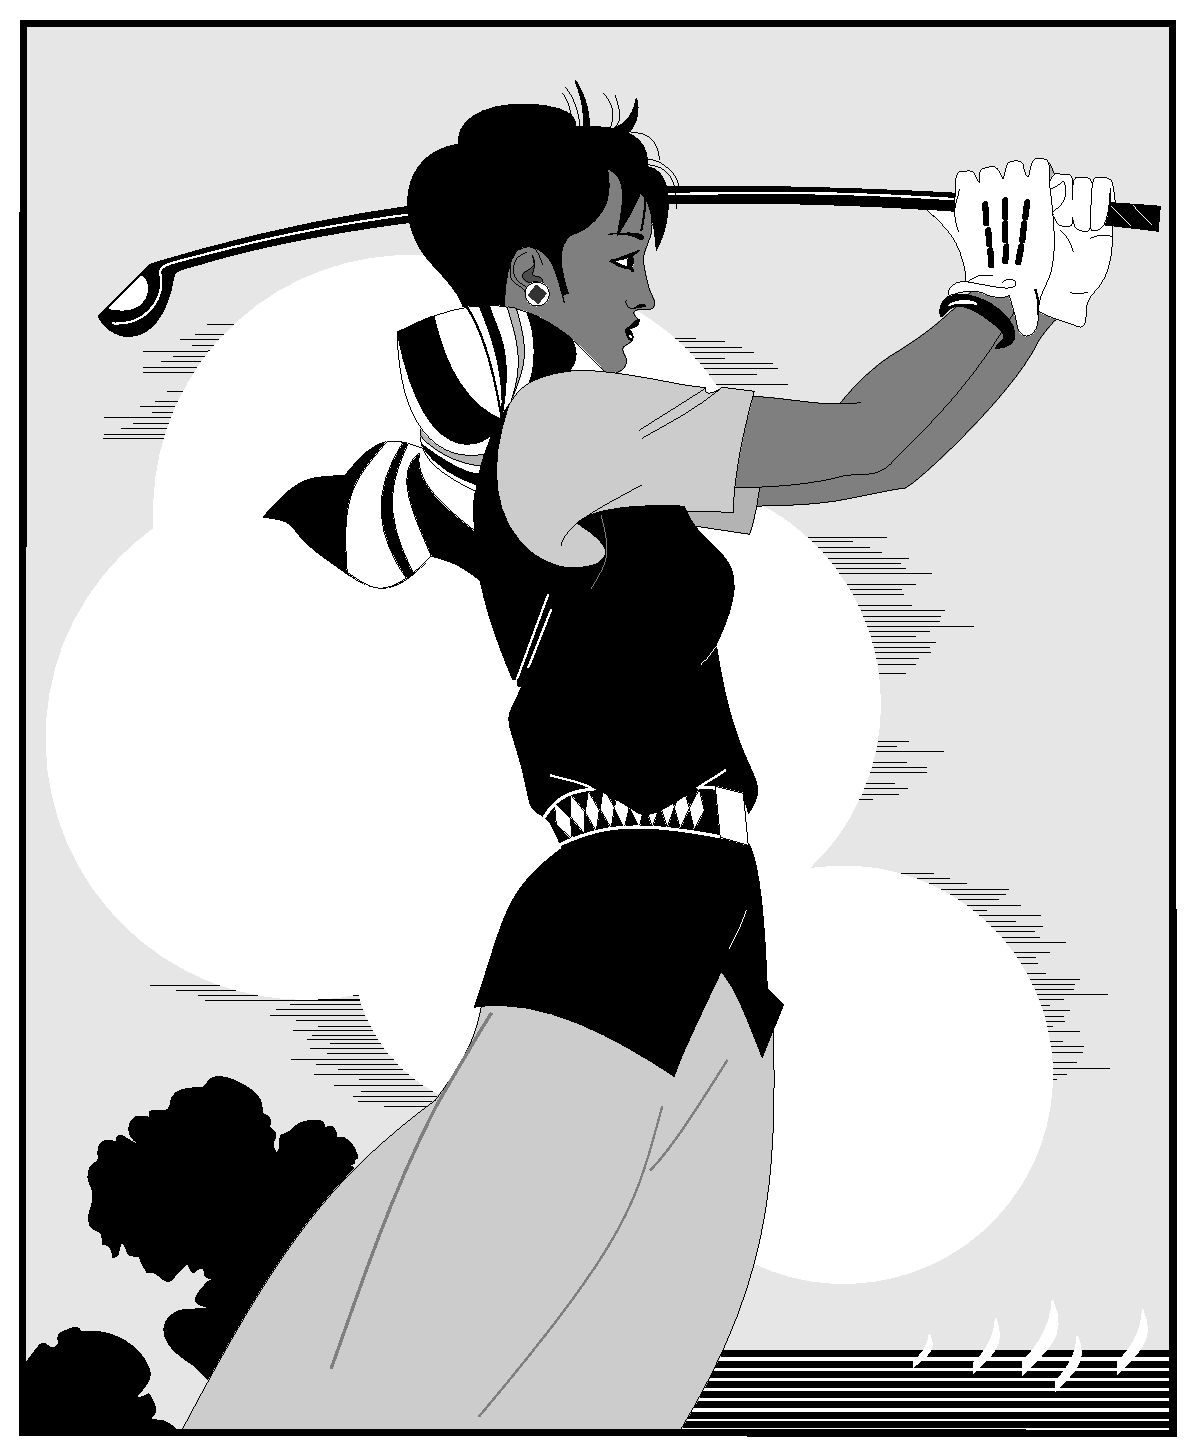
\includegraphics[width=0.2\textwidth]{golfer}}
			\fbox{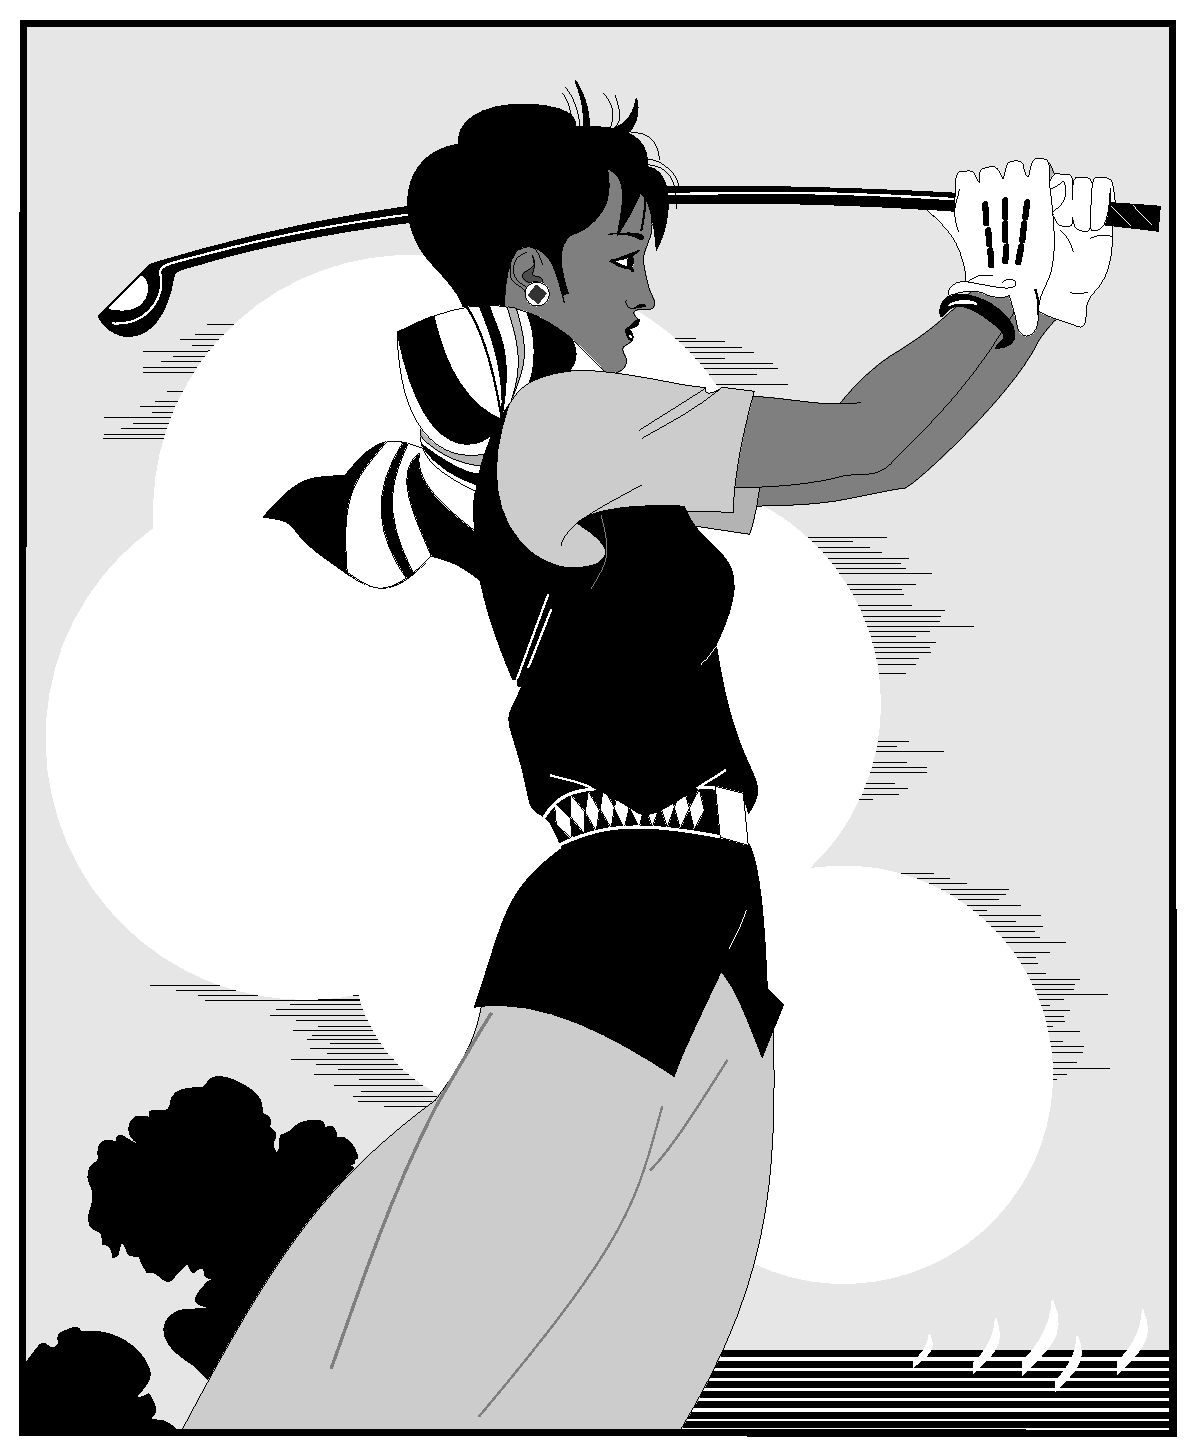
\includegraphics[width=0.2\textwidth]{golfer}}
			\fbox{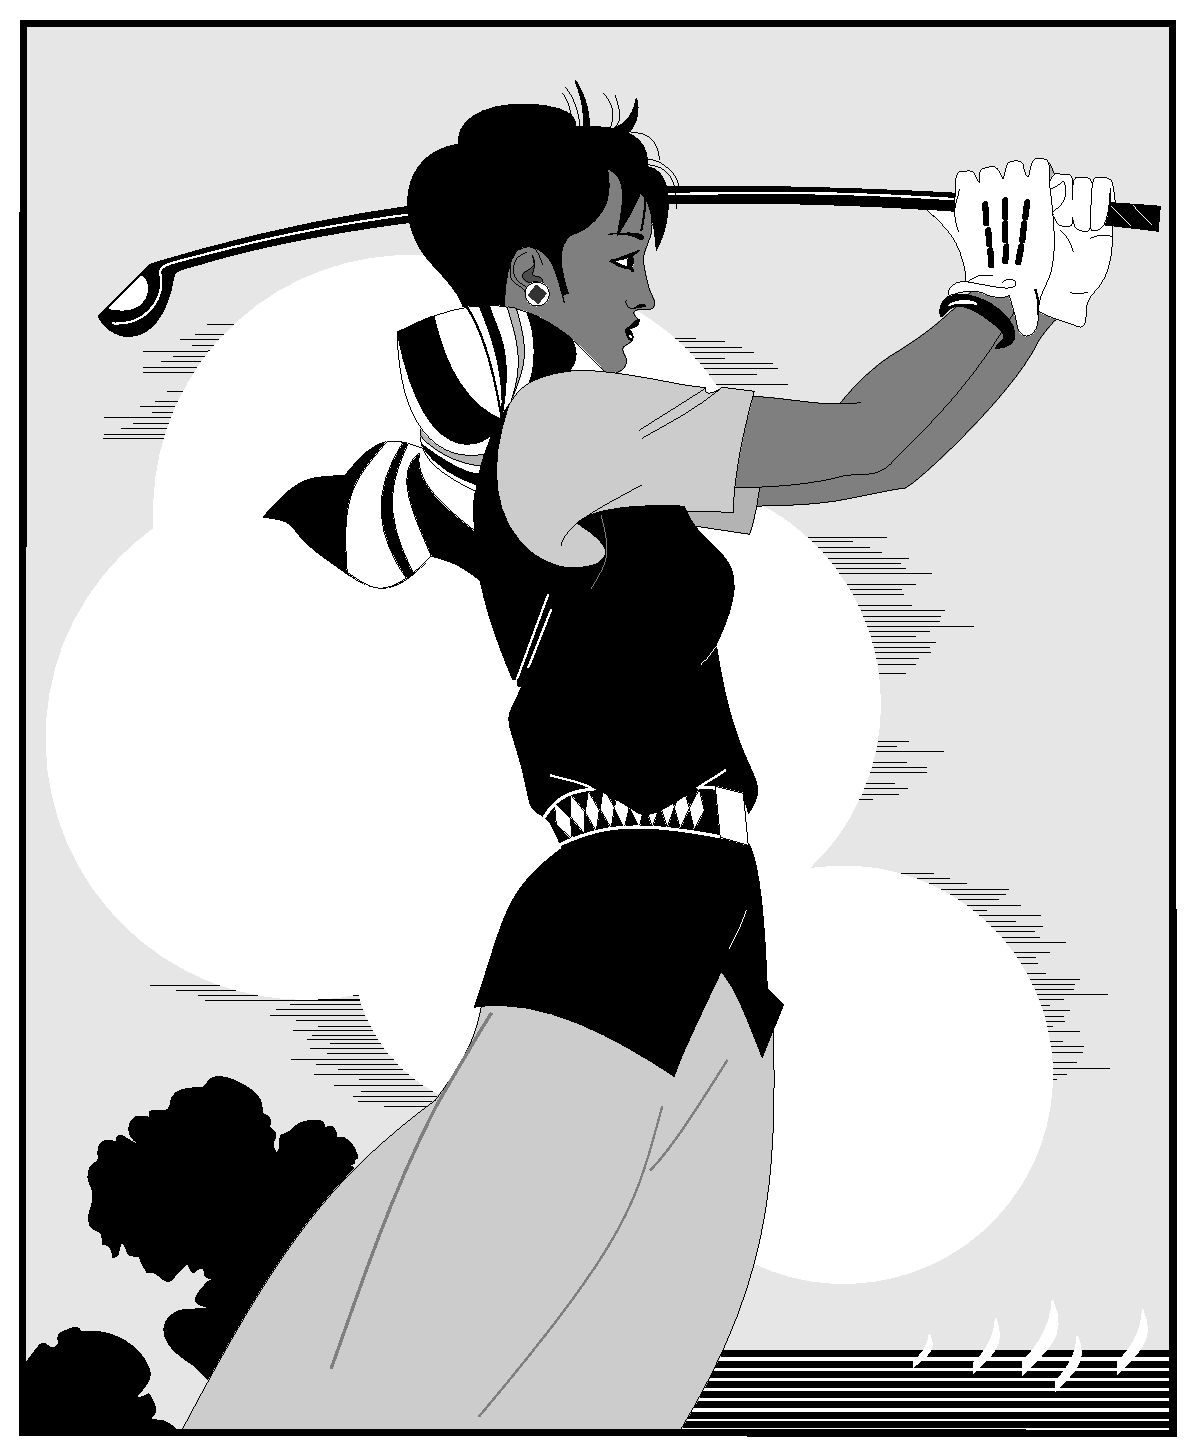
\includegraphics[width=0.2\textwidth]{golfer}}
\bicaption[golfer7]{}{打高尔夫球的人(非规范要求)}{Fig.$\!$}{The person playing golf (Not stated in the regulation)}
		\end{minipage}
	\end{sideways}
\end{figure}

\clearpage

如果不想让图片浮动到下一章节,那么在此处使用\cs{clearpage}命令。

\section{如何做出符合规范的漂亮的图}
关于作图工具在后文\ref{drawtool}中给出一些作图工具的介绍,此处不多言。
此处以R语言和Tikz为例说明如何做出符合规范的图。

\subsection{Tikz作图举例}
使用Tikz作图核心思想是把格式、主题、样式与内容分离,定义在全局中。
注意字体设置可以有两种选择,如何字少,用五号字,字多用小五。
使用Tikz作图不会出现字体问题,字体会自动与正文一致。

\begin{figure}[thb!]
  \centering
      \begin{tikzpicture}[xscale=0.8,yscale=0.3,rotate=90]
        \small
	\draw (-22,6.5) node[refcell]{参考基因组};
	\draw[refline] (-23, 5) -- (27, 5);
	\draw (-22,3.75) node[tscell]{肿瘤样本};
	\draw (-20,3.75) node[tncell]{正常细胞};
	\draw[tnline] (-21, 2.5) -- (27, 2.5);
	\draw (-20,1.25) node[ttcell]{肿瘤细胞};
	\rcell{2}{6};
	\draw[fakeevolve] (4.5, 5.25) -- (4.5, 4.8);
	\ncell{2}{4};
	\draw[evolve] (4.5, 3) .. controls (4.5,2.8) and (-3.5,2.9) ..  (-3.5, 2);
	\draw[evolve] (4.5, 3) .. controls (4.5,2.8) and (11.5,2.9) .. (11.5, 2);
	\tcellone{-6}{1.5};
	\draw (-9, 2) node[ttcell]{1};
	\draw[evolve] (-3.5, 0) .. controls (-3.5,-0.2) and (-12,-0.1) .. (-12, -1.5);
	\draw[evolve] (-3.5, 0) .. controls (-3.5,-0.2) and (1.5,-0.1) .. (1.5, -1.5);
	\tcellthree{7}{1.5};
	\draw (4, 2) node[ttcell]{2};
	\draw[evolve] (11, 0.5) .. controls (11,0.3) and (19,0.4) .. (19, -1.5);
	\tcellfive{-16}{-2};
	\draw (-19, -1.5) node[ttcell]{3};
	\tcelltwo{-1}{-2};
	\draw (-4, -1.5) node[ttcell]{4};
	\tcellfour{12}{-2};
	\draw (9, -1.5) node[ttcell]{5};
      \end{tikzpicture}
  \begin{minipage}{.9\linewidth}
      \vskip 0.2em
      \wuhao 图中,带有箭头的淡蓝色箭头表示肿瘤子种群的进化方向。一般地,从肿瘤组织中取用于进行二代测序的样本中含有一定程度的正常细胞污染,因此肿瘤的样本中含有正常细胞和肿瘤细胞。每一个子种群的基因组的模拟过程是把生殖细胞变异和体细胞变异加入到参考基因组中。
      \vspace{0.6em}
  \end{minipage}
\bicaption[tumor]{}{肿瘤组织中各个子种群的进化示意图}{Fig.$\!$}{The diagram of tumor subpopulation evolution process}
\end{figure}

\subsection{R作图}
R是一种极具有代表性的典型的作图工具,应用广泛。
与Tikz图~\ref{tumor}~不同,R作图分两种情况:(1)可以转换为Tikz码;(2)不可转换为Tikz码。
第一种情况图形简单,图形中不含有很多数据点,使用R语言中的Tikz包即可。
第二种情况是图形复杂,含有海量数据点,这时候不要转成Tikz矢量图,这会使得论文体积巨大。
推荐使用pdf或png非矢量图形。
使用非矢量图形时要注意选择好字号(五号或小五),和字体(宋体、新罗马)然后选择生成图形大小,注意此时在正文中使用\cs{includegraphics}命令导入时,不要像导入矢量图那样控制图形大小,使用图形的原本的
宽度和高度,这样就确保了非矢量图形中的文字与正文一致了。

为了控制\hithesis\ 的大小,此处不给出具体举例,

\section{表格}

表应有自明性。表格不加左、右边线。表的编排建议采用国际通行的三线表。表中文字用宋
体~5~号字。每个表格均应有表题(由表序和表名组成)。表序一般按章编排,如第~1~章第
一个插表的序号为“表~1-1”等。表序与表名之间空一格,表名中不允许使用标点符号,表名
后不加标点。表题置于表上,硕士学位论文只用中文,博士学位论文用中、英文两种文字居
中排写,中文在上,要求中文用宋体~5~号字,英文用新罗马字体~5~号字。表头设计应简单
明了,尽量不用斜线。表头中可采用化学符号或物理量符号。


\subsection{普通表格的绘制方法}[Methods of drawing normal tables]

表格应具有三线表格式,因此需要调用~booktabs~宏包,其标准格式如表~\ref{table1}~所示。
\begin{table}[htbp]
\bicaption[table1]{}{符合研究生院绘图规范的表格}{Table$\!$}{Table in agreement of the standard from graduate school}
\vspace{0.5em}\centering\wuhao
\begin{tabular}{ccccc}
\toprule[1.5pt]
$D$(in) & $P_u$(lbs) & $u_u$(in) & $\beta$ & $G_f$(psi.in)\\
\midrule[1pt]
 5 & 269.8 & 0.000674 & 1.79 & 0.04089\\
10 & 421.0 & 0.001035 & 3.59 & 0.04089\\
20 & 640.2 & 0.001565 & 7.18 & 0.04089\\
\bottomrule[1.5pt]
\end{tabular}
\end{table}
全表如用同一单位,则将单位符号移至表头右上角,加圆括号。表中数据应准确无误,书写
清楚。数字空缺的格内加横线“-”(占~2~个数字宽度)。表内文字或数字上、下或左、右
相同时,采用通栏处理方式,不允许用“〃”、“同上”之类的写法。表内文字说明,起行空一
格、转行顶格、句末不加标点。如某个表需要转页接排,在随后的各页上应重复表的编号。
编号后加“(续表)”,表题可省略。续表应重复表头。

\subsection{长表格的绘制方法}[Methods of drawing long tables]

长表格是当表格在当前页排不下而需要转页接排的情况下所采用的一种表格环境。若长表格
仍按照普通表格的绘制方法来获得,其所使用的\verb|table|浮动环境无法实现表格的换页
接排功能,表格下方过长部分会排在表格第1页的页脚以下。为了能够实现长表格的转页接
排功能,需要调用~longtable~宏包,由于长表格是跨页的文本内容,因此只需要单独的
\verb|longtable|环境,所绘制的长表格的格式如表~\ref{table2}~所示。

注意,长表格双语标题的格式。

\vspace{-1.5bp}
\ltfontsize{\wuhao[1.667]}
\wuhao[1.667]\begin{longtable}{ccc}%
\longbionenumcaption{}{{\wuhao 中国省级行政单位一览
}\label{table3}}{Table$\!$}{}{{\wuhao Overview of the provincial administrative
unit of China}}{-0.5em}{3.15bp}\\
%\caption{\wuhao 中国省级行政单位一览}\\
\toprule[1.5pt] 名称 & 简称 & 省会或首府  \\ \midrule[1pt]
\endfirsthead
\multicolumn{3}{r}{表~\thetable(续表)}\vspace{0.5em}\\
\toprule[1.5pt] 名称 & 简称 & 省会或首府  \\ \midrule[1pt]
\endhead
\bottomrule[1.5pt]
\endfoot
北京市 & 京 & 北京\\
天津市 & 津 & 天津\\
河北省 & 冀 & 石家庄市\\
山西省 & 晋 & 太原市\\
内蒙古自治区 & 蒙 & 呼和浩特市\\
辽宁省 & 辽 & 沈阳市\\
吉林省 & 吉 & 长春市\\
黑龙江省 & 黑 & 哈尔滨市\\
上海市 & 沪/申 & 上海\\
江苏省 & 苏 & 南京市\\
浙江省 & 浙 & 杭州市\\
安徽省 & 皖 & 合肥市\\
福建省 & 闽 & 福州市\\
江西省 & 赣 & 南昌市\\
山东省 & 鲁 & 济南市\\
河南省 & 豫 & 郑州市\\
湖北省 & 鄂 & 武汉市\\
湖南省 & 湘 & 长沙市\\
广东省 & 粤 & 广州市\\
广西壮族自治区 & 桂 & 南宁市\\
海南省 & 琼 & 海口市\\
重庆市 & 渝 & 重庆\\
四川省 & 川/蜀 & 成都市\\
贵州省 & 黔/贵 & 贵阳市\\
云南省 & 云/滇 & 昆明市\\
西藏自治区 & 藏 & 拉萨市\\
陕西省 & 陕/秦 & 西安市\\
甘肃省 & 甘/陇 & 兰州市\\
青海省 & 青 & 西宁市\\
宁夏回族自治区 & 宁 & 银川市\\
新疆维吾尔自治区 & 新 & 乌鲁木齐市\\
香港特别行政区 & 港 & 香港\\
澳门特别行政区 & 澳 & 澳门\\
台湾省 & 台 & 台北市\\
\end{longtable}\normalsize
\vspace{-1em}

此长表格~\ref{table2}~第~2~页的标题“编号(续表)”和表头是通过代码自动添加上去的,无需人工添加,若表格在页面中的竖直位置发生了变化,长表格在第~2~页
及之后各页的标题和表头位置能够始终处于各页的最顶部,也无需人工调整,\LaTeX~系统的这一优点是~word~等软件所无法比拟的。

\subsection{列宽可调表格的绘制方法}[Methods of drawing tables with adjustable-width columns]
论文中能用到列宽可调表格的情况共有两种,一种是当插入的表格某一单元格内容过长以至
于一行放不下的情况,另一种是当对公式中首次出现的物理量符号进行注释的情况,这两种
情况都需要调用~tabularx~宏包。下面将分别对这两种情况下可调表格的绘制方法进行阐述
。
\subsubsection{表格内某单元格内容过长的情况}[The condition when the contents in
some cells of tables are too long]
首先给出这种情况下的一个例子如表~\ref{table3}~所示。
\begin{table}[htbp]
  \centering
\bicaption[table4]{}{最小的三个正整数的英文表示法}{Table$\!$}{The English construction of the smallest three positive integral numbers}\vspace{0.5em}\wuhao
\begin{tabularx}{0.7\textwidth}{llX}
\toprule[1.5pt]
Value & Name & Alternate names, and names for sets of the given size\\\midrule[1pt]
1 & One & ace, single, singleton, unary, unit, unity\\
2 & Two & binary, brace, couple, couplet, distich, deuce, double, doubleton, duad, duality, duet, duo, dyad, pair, snake eyes, span, twain, twosome, yoke\\
3 & Three & deuce-ace, leash, set, tercet, ternary, ternion, terzetto, threesome, tierce, trey, triad, trine, trinity, trio, triplet, troika, hat-trick\\\bottomrule[1.5pt]
\end{tabularx}
\end{table}
tabularx环境共有两个必选参数:第1个参数用来确定表格的总宽度,第2个参数用来确定每
列格式,其中标为X的项表示该列的宽度可调,其宽度值由表格总宽度确定。标为X的列一般
选为单元格内容过长而无法置于一行的列,这样使得该列内容能够根据表格总宽度自动分行
。若列格式中存在不止一个X项,则这些标为X的列的列宽相同,因此,一般不将内容较短的
列设为X。标为X的列均为左对齐,因此其余列一般选为l(左对齐),这样可使得表格美观
,但也可以选为c或r。

\subsubsection{对物理量符号进行注释的情况}[The condition when physical symbols
need to be annotated]

为使得对公式中物理量符号注释的转行与破折号“———”后第一个字对齐,此处最好采用表格
环境。此表格无任何线条,左对齐,且在破折号处对齐,一共有“式中”二字、物理量符号和
注释三列,表格的总宽度可选为文本宽度,因此应该采用\verb|tabularx|环境。由
\verb|tabularx|环境生成的对公式中物理量符号进行注释的公式如式(\ref{eq:1})所示。
\begin{equation}\label{eq:1}
\ddot{\boldsymbol{\rho}}-\frac{\mu}{R_{t}^{3}}\left(3\mathbf{R_{t}}\frac{\mathbf{R_{t}\rho}}{R_{t}^{2}}-\boldsymbol{\rho}\right)=\mathbf{a}
\end{equation}
\begin{tabularx}{\textwidth}{@{}l@{\quad}r@{———}X@{}}
式中& $\boldsymbol{\rho}$ &追踪飞行器与目标飞行器之间的相对位置矢量;\\
&  $\boldsymbol{\ddot{\rho}}$&追踪飞行器与目标飞行器之间的相对加速度;\\
&  $\mathbf{a}$   &推力所产生的加速度;\\
&  $\mathbf{R_t}$ & 目标飞行器在惯性坐标系中的位置矢量;\\
&  $\omega_{t}$ & 目标飞行器的轨道角速度;\\
&  $\mathbf{g}$ & 重力加速度,$=\frac{\mu}{R_{t}^{3}}\left(
3\mathbf{R_{t}}\frac{\mathbf{R_{t}\rho}}{R_{t}^{2}}-\boldsymbol{\rho}\right)=\omega_{t}^{2}\frac{R_{t}}{p}\left(
3\mathbf{R_{t}}\frac{\mathbf{R_{t}\rho}}{R_{t}^{2}}-\boldsymbol{\rho}\right)$,这里~$p$~是目标飞行器的轨道半通径。
\end{tabularx}\vspace{3.15bp}
由此方法生成的注释内容应紧邻待注释公式并置于其下方,因此不能将代码放入
\verb|table|浮动环境中。但此方法不能实现自动转页接排,可能会在当前页剩余空间不够
时,全部移动到下一页而导致当前页出现很大空白。因此在需要转页处理时,还请您手动将
需要转页的代码放入一个新的\verb|tabularx|环境中,将原来的一个\verb|tabularx|环境
拆分为两个\verb|tabularx|环境。

\subsubsection{排版横版表格的举例}[An example of landscape table]

\begin{table}[p]
\centering
\begin{sideways}
\begin{minipage}{\textheight}
\bicaption[table2]{}{不在规范中规定的横版表格}{Table$\!$}{A table style which is not stated in the regulation}
\vspace{0.5em}\centering\wuhao
\begin{tabular}{ccccc}
\toprule[1.5pt]
$D$(in) & $P_u$(lbs) & $u_u$(in) & $\beta$ & $G_f$(psi.in)\\
\midrule[1pt]
 5 & 269.8 & 0.000674 & 1.79 & 0.04089\\
10 & 421.0 & 0.001035 & 3.59 & 0.04089\\
20 & 640.2 & 0.001565 & 7.18 & 0.04089\\
\bottomrule[1.5pt]
\end{tabular}
\end{minipage}
\end{sideways}
\end{table}


\section{公式}
与正常\LaTeX\ 使用方法一致,此处略。关于公式中符号样式的定义在`hithesis.sty'有示
例。

\section{其他杂项}[Miscellaneous]

\subsection{右翻页}[Open right]

对于双面打印的论文,强制使每章的标题页出现右手边为右翻页。
规范中没有明确规定是否是右翻页打印。
模板给出了右翻页选项。
为了应对用户的个人喜好,在希望设置成右翻页的位置之前添加\cs{cleardoublepage}命令即可。

\subsection{算法}[Algorithms]
我工算法有以下几大特点。

(1)算法不在规范中要求。

(2)算法常常被使用(至少计算机学院)。

(3)格式乱,甚至出现了每个实验室的格式要求都不一样。

此处不给出示例,因为没法给,在
\href{https://github.com/dustincys/PlutoThesis}{https://github.com/dustincys/PlutoThesis}
的readme文件中有不同实验室算法要求说明。

\subsection{脚注}[Footnotes]
不在再规范\footnote{规范是指\PGR\ 和\UGR}中要求,模板默认使用清华大学的格式。

\subsection{源码}[Source code]
也不在再规范中要求。如果有需要最好使用minted包,但在编译的时候需要添加“
-shell-escape”选项且安装pygmentize软件,这些不在模板中默认载入,如果需要自行载入
。
\subsection{思源宋体}[Siyuan font]
如果要使用思源字体,需要思源字体的定义文件,此文件请到模板的开发版网址github:
\href{https://gihitb.com/dustincys/hithesis}{https://gihitb.com/dustincys/hithesis}
或者oschia:
\href{https://git.oschina.net/dustincys/hithesis}{https://git.oschina.net/dustincys/hithesis}
处下载。

\subsection{专业绘图工具}[Processional drawing tool]
\label{drawtool}
推荐使用tikz包,使用tikz源码绘图的好处是,图片中的字体与正文中的字体一致。具体如
何使用tikz绘图不属于模板范畴。
tikz适合用来画不需要大量实验数据支撑示意图。但R语言等专业绘图工具具有画出各种、
专业、复杂的数据图。R语言中有tikz包,能自动生成tikz码,这样tikz几乎无所不能。
对于排版有极致追求的小伙伴,可以参考
\href{http://www.texample.net/tikz/resources/}{http://www.texample.net/tikz/resources/}
中所列工具,几乎所有作图软件所作的图形都可转成tikz,然后可以自由的在tikz中修改
图中内容,定义字体等等。实现前文窝工规范中要求的图中字体的一致性的终极目标。


\subsection{术语词汇管理}[Manage glossaries]
推荐使用glossaries包管理术语、缩略语,可以自动生成首次全写,非首次缩写。

\subsection{\TeX\ 源码编辑器}[\TeX editor]
推荐:(1)付费软件Winedt;(2)免费软件kile;(3)vim或emaces或sublime等神级编
译器(需要配置)。

\subsection{\LaTeX\ 排版重要原则}[\LaTeX\ typesetting rules]
格式和内容分离是\LaTeX\ 最大优势,所有多次出现的内容、样式等等都可以定义为简单命
令、环境。这样的好处是方便修改、管理。例如,如果想要把所有的表示向量的符号由粗体
\cs{mathbf}变换到花体\cs{mathcal},只需修改该格式的命令的定义部分,不需要像MS
word那样处处修改。总而言之,使用自定义命令和环境才是正确的使用\LaTeX\ 的方式。

\section{关于捐助}
各位刀客和大侠如用的嗨,要解囊相助,请参照图~\ref{zfb}~中提示操作(二维码被矢量化后之后去
除了头像等冗余无用的部分~)。

\begin{figure}[!h]
\centering\includegraphics[width=0.4\textwidth]{zfb}
\vspace{0.2em}
\bicaption[Donation]{}{捐助,注意此处是子图只用汉语图题的形式,我工规定可以不用
英语图题}{Fig.$\!$}{Donation, please note that it is OK to use Chinese caption
only}
\end{figure}


% Local Variables:
% TeX-master: "../main"
% TeX-engine: xetex
% End:
